\documentclass[twoside]{book}

% Packages required by doxygen
\usepackage{fixltx2e}
\usepackage{calc}
\usepackage{doxygen}
\usepackage[export]{adjustbox} % also loads graphicx
\usepackage{graphicx}
\usepackage[utf8]{inputenc}
\usepackage{makeidx}
\usepackage{multicol}
\usepackage{multirow}
\PassOptionsToPackage{warn}{textcomp}
\usepackage{textcomp}
\usepackage[nointegrals]{wasysym}
\usepackage[table]{xcolor}

% NLS support packages
\usepackage[french]{babel}

% Font selection
\usepackage[T1]{fontenc}
\usepackage[scaled=.90]{helvet}
\usepackage{courier}
\usepackage{amssymb}
\usepackage{sectsty}
\renewcommand{\familydefault}{\sfdefault}
\allsectionsfont{%
  \fontseries{bc}\selectfont%
  \color{darkgray}%
}
\renewcommand{\DoxyLabelFont}{%
  \fontseries{bc}\selectfont%
  \color{darkgray}%
}
\newcommand{\+}{\discretionary{\mbox{\scriptsize$\hookleftarrow$}}{}{}}

% Page & text layout
\usepackage{geometry}
\geometry{%
  a4paper,%
  top=2.5cm,%
  bottom=2.5cm,%
  left=2.5cm,%
  right=2.5cm%
}
\tolerance=750
\hfuzz=15pt
\hbadness=750
\setlength{\emergencystretch}{15pt}
\setlength{\parindent}{0cm}
\setlength{\parskip}{0.2cm}
\makeatletter
\renewcommand{\paragraph}{%
  \@startsection{paragraph}{4}{0ex}{-1.0ex}{1.0ex}{%
    \normalfont\normalsize\bfseries\SS@parafont%
  }%
}
\renewcommand{\subparagraph}{%
  \@startsection{subparagraph}{5}{0ex}{-1.0ex}{1.0ex}{%
    \normalfont\normalsize\bfseries\SS@subparafont%
  }%
}
\makeatother

% Headers & footers
\usepackage{fancyhdr}
\pagestyle{fancyplain}
\fancyhead[LE]{\fancyplain{}{\bfseries\thepage}}
\fancyhead[CE]{\fancyplain{}{}}
\fancyhead[RE]{\fancyplain{}{\bfseries\leftmark}}
\fancyhead[LO]{\fancyplain{}{\bfseries\rightmark}}
\fancyhead[CO]{\fancyplain{}{}}
\fancyhead[RO]{\fancyplain{}{\bfseries\thepage}}
\fancyfoot[LE]{\fancyplain{}{}}
\fancyfoot[CE]{\fancyplain{}{}}
\fancyfoot[RE]{\fancyplain{}{\bfseries\scriptsize Généré le Lundi 28 Septembre 2015 00\+:51\+:38 pour Terrain tracing par Doxygen }}
\fancyfoot[LO]{\fancyplain{}{\bfseries\scriptsize Généré le Lundi 28 Septembre 2015 00\+:51\+:38 pour Terrain tracing par Doxygen }}
\fancyfoot[CO]{\fancyplain{}{}}
\fancyfoot[RO]{\fancyplain{}{}}
\renewcommand{\footrulewidth}{0.4pt}
\renewcommand{\chaptermark}[1]{%
  \markboth{#1}{}%
}
\renewcommand{\sectionmark}[1]{%
  \markright{\thesection\ #1}%
}

% Indices & bibliography
\usepackage{natbib}
\usepackage[titles]{tocloft}
\setcounter{tocdepth}{3}
\setcounter{secnumdepth}{5}
\makeindex

% Hyperlinks (required, but should be loaded last)
\usepackage{ifpdf}
\ifpdf
  \usepackage[pdftex,pagebackref=true]{hyperref}
\else
  \usepackage[ps2pdf,pagebackref=true]{hyperref}
\fi
\hypersetup{%
  colorlinks=true,%
  linkcolor=blue,%
  citecolor=blue,%
  unicode%
}

% Custom commands
\newcommand{\clearemptydoublepage}{%
  \newpage{\pagestyle{empty}\cleardoublepage}%
}


%===== C O N T E N T S =====

\begin{document}

% Titlepage & ToC
\hypersetup{pageanchor=false,
             bookmarks=true,
             bookmarksnumbered=true,
             pdfencoding=unicode
            }
\pagenumbering{roman}
\begin{titlepage}
\vspace*{7cm}
\begin{center}%
{\Large Terrain tracing }\\
\vspace*{1cm}
{\large Généré par Doxygen 1.8.10}\\
\vspace*{0.5cm}
{\small Lundi 28 Septembre 2015 00:51:38}\\
\end{center}
\end{titlepage}
\clearemptydoublepage
\tableofcontents
\clearemptydoublepage
\pagenumbering{arabic}
\hypersetup{pageanchor=true}

%--- Begin generated contents ---
\chapter{Index des espaces de nommage}
\section{Liste des espaces de nommage}
Liste de tous les espaces de nommage documentés avec une brève description\+:\begin{DoxyCompactList}
\item\contentsline{section}{\hyperlink{namespacenrw}{nrw} }{\pageref{namespacenrw}}{}
\end{DoxyCompactList}

\chapter{Index hiérarchique}
\section{Hiérarchie des classes}
Cette liste d\textquotesingle{}héritage est classée approximativement par ordre alphabétique \+:\begin{DoxyCompactList}
\item \contentsline{section}{Box}{\pageref{class_box}}{}
\item \contentsline{section}{Camera}{\pageref{class_camera}}{}
\item \contentsline{section}{Color\+Gradient}{\pageref{class_color_gradient}}{}
\item \contentsline{section}{Color\+Gradient\+:\+:Color\+Point}{\pageref{struct_color_gradient_1_1_color_point}}{}
\item \contentsline{section}{Lumiere}{\pageref{class_lumiere}}{}
\item \contentsline{section}{Mesh}{\pageref{class_mesh}}{}
\item \contentsline{section}{Rayon}{\pageref{class_rayon}}{}
\item \contentsline{section}{Scene}{\pageref{class_scene}}{}
\item \contentsline{section}{Terrain}{\pageref{class_terrain}}{}
\begin{DoxyCompactList}
\item \contentsline{section}{Terrain\+Noise}{\pageref{class_terrain_noise}}{}
\item \contentsline{section}{Terrain\+Tab}{\pageref{class_terrain_tab}}{}
\end{DoxyCompactList}
\end{DoxyCompactList}

\chapter{Index des classes}
\section{Liste des classes}
Liste des classes, structures, unions et interfaces avec une brève description \+:\begin{DoxyCompactList}
\item\contentsline{section}{\hyperlink{class_box}{Box} \\*Classe d\textquotesingle{}un objet géométrique de type boite. ~\newline
 Il sert de boite englobante pour les objets }{\pageref{class_box}}{}
\item\contentsline{section}{\hyperlink{class_camera}{Camera} \\*Une caméra utilisé pour visualiser la scène }{\pageref{class_camera}}{}
\item\contentsline{section}{\hyperlink{class_color_gradient}{Color\+Gradient} \\*Class containing multiple color and perform a gradient on this color }{\pageref{class_color_gradient}}{}
\item\contentsline{section}{\hyperlink{struct_color_gradient_1_1_color_point}{Color\+Gradient\+::\+Color\+Point} \\*Internal class used to store colors at different points in the gradient }{\pageref{struct_color_gradient_1_1_color_point}}{}
\item\contentsline{section}{\hyperlink{class_lumiere}{Lumiere} }{\pageref{class_lumiere}}{}
\item\contentsline{section}{\hyperlink{class_mesh}{Mesh} }{\pageref{class_mesh}}{}
\item\contentsline{section}{\hyperlink{class_rayon}{Rayon} \\*Classe représentant un rayon lumineux }{\pageref{class_rayon}}{}
\item\contentsline{section}{\hyperlink{class_scene}{Scene} \\*Correspond à un scène dans sa globalité }{\pageref{class_scene}}{}
\item\contentsline{section}{\hyperlink{class_terrain}{Terrain} \\*Classe virtuelle de terrain. Sert de modèle pour les classes files \hyperlink{class_terrain_noise}{Terrain\+Noise} et \hyperlink{class_terrain_tab}{Terrain\+Tab} }{\pageref{class_terrain}}{}
\item\contentsline{section}{\hyperlink{class_terrain_noise}{Terrain\+Noise} \\*Classe fille de \hyperlink{class_terrain}{Terrain}. Elle s\textquotesingle{}appuis sur l\textquotesingle{}utilisation de noise pour déterminer la forme du terrain }{\pageref{class_terrain_noise}}{}
\item\contentsline{section}{\hyperlink{class_terrain_tab}{Terrain\+Tab} \\*Classe fille de \hyperlink{class_terrain}{Terrain}. Elle s\textquotesingle{}appuis sur l\textquotesingle{}utilisation d\textquotesingle{}un image High\+Map pour déterminer la forme du terrain }{\pageref{class_terrain_tab}}{}
\end{DoxyCompactList}

\chapter{Documentation des espaces de nommage}
\hypertarget{namespacenrw}{}\section{Référence de l\textquotesingle{}espace de nommage nrw}
\label{namespacenrw}\index{nrw@{nrw}}
\subsection*{Fonctions}
\begin{DoxyCompactItemize}
\item 
float \hyperlink{namespacenrw_a1e69bf74e7416ba334580e4b12bc7a57}{noise} (int amplitude, float periode, float x, float y)
\begin{DoxyCompactList}\small\item\em Récupération d\textquotesingle{}une valeur de noise suivant les paramétres donnés. \end{DoxyCompactList}\item 
float \hyperlink{namespacenrw_a50a0ba8cc607beb2bed090e356e888ba}{ridge} (float hauteur, float seuil)
\item 
float \hyperlink{namespacenrw_a83e556a2082b0e965aaddcc2ab74f576}{attenuation} (float h, float min, float max)
\begin{DoxyCompactList}\small\item\em Terrain\+::attenuation. \end{DoxyCompactList}\end{DoxyCompactItemize}


\subsection{Description détaillée}

\begin{DoxyParams}{Paramètres}
{\em fonction} & pour noise, ridge, warp et toutes fonction sur le terrain qui n\textquotesingle{}ont pas besoin de connaitre les caractéristiques du terrain \\
\hline
\end{DoxyParams}


\subsection{Documentation des fonctions}
\hypertarget{namespacenrw_a83e556a2082b0e965aaddcc2ab74f576}{}\index{nrw@{nrw}!attenuation@{attenuation}}
\index{attenuation@{attenuation}!nrw@{nrw}}
\subsubsection[{attenuation(float h, float min, float max)}]{\setlength{\rightskip}{0pt plus 5cm}float nrw\+::attenuation (
\begin{DoxyParamCaption}
\item[{float}]{h, }
\item[{float}]{min, }
\item[{float}]{max}
\end{DoxyParamCaption}
)}\label{namespacenrw_a83e556a2082b0e965aaddcc2ab74f576}


Terrain\+::attenuation. 


\begin{DoxyParams}[1]{Paramètres}
\mbox{\tt in}  & {\em h} & valeur que l\textquotesingle{}on souhaite atténuer \\
\hline
\mbox{\tt in}  & {\em min} & seuil minimum à partir duquel la fonctin renvoie un résulttat $>$ à 0 \\
\hline
\mbox{\tt in}  & {\em max} & seuil à partir duquel la fonction renvoie toujours 1 \\
\hline
\end{DoxyParams}
\begin{DoxyReturn}{Renvoie}
Un coefficient entre 0 et 1 dépendant de l\textquotesingle{}élévation 
\end{DoxyReturn}
\hypertarget{namespacenrw_a1e69bf74e7416ba334580e4b12bc7a57}{}\index{nrw@{nrw}!noise@{noise}}
\index{noise@{noise}!nrw@{nrw}}
\subsubsection[{noise(int amplitude, float periode, float x, float y)}]{\setlength{\rightskip}{0pt plus 5cm}float nrw\+::noise (
\begin{DoxyParamCaption}
\item[{int}]{amplitude, }
\item[{float}]{periode, }
\item[{float}]{x, }
\item[{float}]{y}
\end{DoxyParamCaption}
)}\label{namespacenrw_a1e69bf74e7416ba334580e4b12bc7a57}


Récupération d\textquotesingle{}une valeur de noise suivant les paramétres donnés. 


\begin{DoxyParams}[1]{Paramètres}
\mbox{\tt in}  & {\em amplitude} & Amplitude max que pourra atteindre le noise. \\
\hline
\mbox{\tt in}  & {\em periode} & Distance en metre pour que le noise atteigne un cycle. \\
\hline
\mbox{\tt in}  & {\em x} & abscisse du terrain (entre 0 et 1). \\
\hline
\mbox{\tt in}  & {\em y} & ordonnée du terrain (entre 0 et 1). \\
\hline
\end{DoxyParams}
\begin{DoxyReturn}{Renvoie}
La valeur générée par le noise. 
\end{DoxyReturn}
\hypertarget{namespacenrw_a50a0ba8cc607beb2bed090e356e888ba}{}\index{nrw@{nrw}!ridge@{ridge}}
\index{ridge@{ridge}!nrw@{nrw}}
\subsubsection[{ridge(float hauteur, float seuil)}]{\setlength{\rightskip}{0pt plus 5cm}float nrw\+::ridge (
\begin{DoxyParamCaption}
\item[{float}]{hauteur, }
\item[{float}]{seuil}
\end{DoxyParamCaption}
)}\label{namespacenrw_a50a0ba8cc607beb2bed090e356e888ba}

\begin{DoxyParams}{Paramètres}
{\em hauteur} & hauteur que l\textquotesingle{}on veut modifier par un ridge \\
\hline
{\em seuil} & hauteur max et de découpe du terrain \\
\hline
\end{DoxyParams}
\begin{DoxyReturn}{Renvoie}
la nouvelle hauteur $<$ seuil 
\end{DoxyReturn}

\chapter{Documentation des classes}
\hypertarget{class_box}{}\section{Référence de la classe Box}
\label{class_box}\index{Box@{Box}}


Classe d\textquotesingle{}un objet géométrique de type boite. ~\newline
 Il sert de boite englobante pour les objets.  




{\ttfamily \#include $<$box.\+h$>$}

\subsection*{Fonctions membres publiques}
\begin{DoxyCompactItemize}
\item 
\hypertarget{class_box_aa232abb63b2b72d93791c74a96ac7de9}{}{\bfseries Box} (const Vector3f \&\+\_\+min, const Vector3f \&\+\_\+max)\label{class_box_aa232abb63b2b72d93791c74a96ac7de9}

\item 
\hyperlink{class_box_a2353559b5ce40e7edcc85daddd86f292}{Box} (const std\+::vector$<$ Vector3f $>$ \&points)
\begin{DoxyCompactList}\small\item\em Constructeur qui utilisera un ensemble de points pour calculer la boite englobante correspondante. ~\newline
Le constructeur passe le relai à la fonction \hyperlink{class_box_a8ffb517da2017677041941e1b2f60f1f}{parcourt\+Points()}. \end{DoxyCompactList}\item 
void \hyperlink{class_box_ad4ee0fca654414f2f9f5092f70ab92e7}{update\+Point} (const Vector3f \&p)
\begin{DoxyCompactList}\small\item\em Détermine si la boite englobante doit être modifiée pour comprendre le point {\itshape p}. ~\newline
Si c\textquotesingle{}est le cas la boite s\textquotesingle{}adapte pour contenir le point. ~\newline
Passe le relai à la méthode \hyperlink{class_box_a13162f123f21923c3b22ba02a2211143}{update()}. \end{DoxyCompactList}\item 
bool \hyperlink{class_box_a2d6c41818d3d77ba71866528f5e6ccac}{is\+In} (const Vector3f \&p) const 
\begin{DoxyCompactList}\small\item\em Test si le point {\itshape p} est dans l\textquotesingle{}espace compris de la boite. \end{DoxyCompactList}\item 
bool \hyperlink{class_box_a6ce97deba91479b4fa66c260c1a37c8a}{intersect} (const \hyperlink{class_rayon}{Rayon} \&r, float \&distance\+Min, float \&distance\+Max) const 
\begin{DoxyCompactList}\small\item\em Test si un rayon traverse la boite. ~\newline
Si c\textquotesingle{}est le cas, la methode retournera les distance d\textquotesingle{}intersection sur la boite. (cf. \hyperlink{class_rayon}{Rayon}) ~\newline
Utilise la méthode \hyperlink{class_box_a54e436e7e487b4a9c75eaf342d430b64}{intersect\+In()}. \end{DoxyCompactList}\item 
float \hyperlink{class_box_a173e401890b2cb5af0ba69d78c9df413}{diff\+Z} () const 
\begin{DoxyCompactList}\small\item\em Calcul la hauteur en {\itshape z} de la boite. \end{DoxyCompactList}\item 
void \hyperlink{class_box_a5aebe0463a5c45d1cf966fbccabef94f}{merge} (const \hyperlink{class_box}{Box} \&box2)
\begin{DoxyCompactList}\small\item\em Fait l\textquotesingle{}union entre deux boites, et redéfini min et max pour englober les deux boites. \end{DoxyCompactList}\item 
void \hyperlink{class_box_a8b1ad9cb82546788f3ad6001429b5c5f}{operator+=} (const Vector3f \&t)
\begin{DoxyCompactList}\small\item\em Opère un translation rectiligne de la boite. \end{DoxyCompactList}\end{DoxyCompactItemize}
\subsection*{Attributs publics}
\begin{DoxyCompactItemize}
\item 
\hypertarget{class_box_a4b5893565a3e2b26361338b19af0671a}{}Vector3f \hyperlink{class_box_a4b5893565a3e2b26361338b19af0671a}{min}\label{class_box_a4b5893565a3e2b26361338b19af0671a}

\begin{DoxyCompactList}\small\item\em min Position d\textquotesingle{}un des points de la boite. \end{DoxyCompactList}\item 
\hypertarget{class_box_ac7d2365a0645043a21a055942019cd74}{}Vector3f \hyperlink{class_box_ac7d2365a0645043a21a055942019cd74}{max}\label{class_box_ac7d2365a0645043a21a055942019cd74}

\begin{DoxyCompactList}\small\item\em max Position du point opposé au point {\itshape min} sur la boite. \end{DoxyCompactList}\end{DoxyCompactItemize}
\subsection*{Fonctions membres privées}
\begin{DoxyCompactItemize}
\item 
\hypertarget{class_box_a411b56ce2f6a9c29e83ce8c16d99adae}{}void \hyperlink{class_box_a411b56ce2f6a9c29e83ce8c16d99adae}{set\+Default\+Box} ()\label{class_box_a411b56ce2f6a9c29e83ce8c16d99adae}

\begin{DoxyCompactList}\small\item\em Initialise la boite avec des valeurs par defaut. \end{DoxyCompactList}\item 
void \hyperlink{class_box_a13162f123f21923c3b22ba02a2211143}{update} (const Vector3f \&p)
\begin{DoxyCompactList}\small\item\em Détermine si la boite englobante doit être modifiée pour comprendre le point {\itshape p}. ~\newline
Si c\textquotesingle{}est le cas la boite s\textquotesingle{}adapte pour contenir le point. ~\newline
Passe le relai à la méthode \hyperlink{class_box_a3aafcee14e1e0ea4a6fe1b61d463fbd5}{update\+Min()} et \hyperlink{class_box_ab637f4c06fd3359557445917f18d4f1f}{update\+Max()}. \end{DoxyCompactList}\item 
void \hyperlink{class_box_a3aafcee14e1e0ea4a6fe1b61d463fbd5}{update\+Min} (const Vector3f \&p)
\begin{DoxyCompactList}\small\item\em Détermine si le point min doit être modifiée pour comprendre le point {\itshape p}. ~\newline
Si c\textquotesingle{}est le cas le point min s\textquotesingle{}adapte pour contenir le point. ~\newline
. \end{DoxyCompactList}\item 
void \hyperlink{class_box_ab637f4c06fd3359557445917f18d4f1f}{update\+Max} (const Vector3f \&p)
\begin{DoxyCompactList}\small\item\em Détermine si le point max doit être modifiée pour comprendre le point {\itshape p}. ~\newline
Si c\textquotesingle{}est le cas le point max s\textquotesingle{}adapte pour contenir le point. ~\newline
. \end{DoxyCompactList}\item 
void \hyperlink{class_box_a8ffb517da2017677041941e1b2f60f1f}{parcourt\+Points} (const std\+::vector$<$ Vector3f $>$ \&points)
\begin{DoxyCompactList}\small\item\em Détermine la positions de min et max pour englober tous les points de {\itshape points}. \end{DoxyCompactList}\item 
float \hyperlink{class_box_a54e436e7e487b4a9c75eaf342d430b64}{intersect\+In} (const \hyperlink{class_rayon}{Rayon} \&r) const 
\begin{DoxyCompactList}\small\item\em Test si le rayon r traverse la boite. \end{DoxyCompactList}\end{DoxyCompactItemize}


\subsection{Description détaillée}
Classe d\textquotesingle{}un objet géométrique de type boite. ~\newline
 Il sert de boite englobante pour les objets. 

\subsection{Documentation des constructeurs et destructeur}
\hypertarget{class_box_a2353559b5ce40e7edcc85daddd86f292}{}\index{Box@{Box}!Box@{Box}}
\index{Box@{Box}!Box@{Box}}
\subsubsection[{Box(const std\+::vector$<$ Vector3f $>$ \&points)}]{\setlength{\rightskip}{0pt plus 5cm}Box\+::\+Box (
\begin{DoxyParamCaption}
\item[{const std\+::vector$<$ Vector3f $>$ \&}]{points}
\end{DoxyParamCaption}
)}\label{class_box_a2353559b5ce40e7edcc85daddd86f292}


Constructeur qui utilisera un ensemble de points pour calculer la boite englobante correspondante. ~\newline
Le constructeur passe le relai à la fonction \hyperlink{class_box_a8ffb517da2017677041941e1b2f60f1f}{parcourt\+Points()}. 


\begin{DoxyParams}[1]{Paramètres}
\mbox{\tt in}  & {\em points} & Tableau de position de points d\textquotesingle{}un objet. \\
\hline
\end{DoxyParams}


\subsection{Documentation des fonctions membres}
\hypertarget{class_box_a173e401890b2cb5af0ba69d78c9df413}{}\index{Box@{Box}!diff\+Z@{diff\+Z}}
\index{diff\+Z@{diff\+Z}!Box@{Box}}
\subsubsection[{diff\+Z() const }]{\setlength{\rightskip}{0pt plus 5cm}float Box\+::diff\+Z (
\begin{DoxyParamCaption}
{}
\end{DoxyParamCaption}
) const}\label{class_box_a173e401890b2cb5af0ba69d78c9df413}


Calcul la hauteur en {\itshape z} de la boite. 

\begin{DoxyReturn}{Renvoie}
la hauteur en {\itshape z}. 
\end{DoxyReturn}
\hypertarget{class_box_a6ce97deba91479b4fa66c260c1a37c8a}{}\index{Box@{Box}!intersect@{intersect}}
\index{intersect@{intersect}!Box@{Box}}
\subsubsection[{intersect(const Rayon \&r, float \&distance\+Min, float \&distance\+Max) const }]{\setlength{\rightskip}{0pt plus 5cm}bool Box\+::intersect (
\begin{DoxyParamCaption}
\item[{const {\bf Rayon} \&}]{r, }
\item[{float \&}]{distance\+Min, }
\item[{float \&}]{distance\+Max}
\end{DoxyParamCaption}
) const}\label{class_box_a6ce97deba91479b4fa66c260c1a37c8a}


Test si un rayon traverse la boite. ~\newline
Si c\textquotesingle{}est le cas, la methode retournera les distance d\textquotesingle{}intersection sur la boite. (cf. \hyperlink{class_rayon}{Rayon}) ~\newline
Utilise la méthode \hyperlink{class_box_a54e436e7e487b4a9c75eaf342d430b64}{intersect\+In()}. 


\begin{DoxyParams}[1]{Paramètres}
\mbox{\tt in}  & {\em r} & Un rayon quelconque. (cf. \hyperlink{class_rayon}{Rayon}) \\
\hline
\mbox{\tt out}  & {\em distance\+Min} & coefficient de distance du premier impacte sur la boite par rapport à l\textquotesingle{}origine du rayon. ~\newline
Le coefficient est dependant de la norme du vecteur direction du rayon. \\
\hline
\mbox{\tt out}  & {\em distance\+Max} & coefficient de distance du second impacte sur la boite par rapport à l\textquotesingle{}origine du rayon. ~\newline
Le coefficient est dependant de la norme du vecteur direction du rayon. \\
\hline
\end{DoxyParams}
\begin{DoxyReturn}{Renvoie}
Le resultat du test. True = intersection, false = pas d\textquotesingle{}intersection. 
\end{DoxyReturn}
\hypertarget{class_box_a54e436e7e487b4a9c75eaf342d430b64}{}\index{Box@{Box}!intersect\+In@{intersect\+In}}
\index{intersect\+In@{intersect\+In}!Box@{Box}}
\subsubsection[{intersect\+In(const Rayon \&r) const }]{\setlength{\rightskip}{0pt plus 5cm}float Box\+::intersect\+In (
\begin{DoxyParamCaption}
\item[{const {\bf Rayon} \&}]{r}
\end{DoxyParamCaption}
) const\hspace{0.3cm}{\ttfamily [inline]}, {\ttfamily [private]}}\label{class_box_a54e436e7e487b4a9c75eaf342d430b64}


Test si le rayon r traverse la boite. 


\begin{DoxyParams}[1]{Paramètres}
\mbox{\tt in}  & {\em r} & Un rayon quelconque. (cf. \hyperlink{class_rayon}{Rayon}) \\
\hline
\end{DoxyParams}
\begin{DoxyReturn}{Renvoie}
Le test d\textquotesingle{}intersection entre la boite et {\itshape r}. 
\end{DoxyReturn}
\hypertarget{class_box_a2d6c41818d3d77ba71866528f5e6ccac}{}\index{Box@{Box}!is\+In@{is\+In}}
\index{is\+In@{is\+In}!Box@{Box}}
\subsubsection[{is\+In(const Vector3f \&p) const }]{\setlength{\rightskip}{0pt plus 5cm}bool Box\+::is\+In (
\begin{DoxyParamCaption}
\item[{const Vector3f \&}]{p}
\end{DoxyParamCaption}
) const}\label{class_box_a2d6c41818d3d77ba71866528f5e6ccac}


Test si le point {\itshape p} est dans l\textquotesingle{}espace compris de la boite. 


\begin{DoxyParams}[1]{Paramètres}
\mbox{\tt in}  & {\em p} & un point dans l\textquotesingle{}espace x, y, z. \\
\hline
\end{DoxyParams}
\begin{DoxyReturn}{Renvoie}
Le resultat du test. True = dedans, false = dehors. 
\end{DoxyReturn}
\hypertarget{class_box_a5aebe0463a5c45d1cf966fbccabef94f}{}\index{Box@{Box}!merge@{merge}}
\index{merge@{merge}!Box@{Box}}
\subsubsection[{merge(const Box \&box2)}]{\setlength{\rightskip}{0pt plus 5cm}void Box\+::merge (
\begin{DoxyParamCaption}
\item[{const {\bf Box} \&}]{box2}
\end{DoxyParamCaption}
)}\label{class_box_a5aebe0463a5c45d1cf966fbccabef94f}


Fait l\textquotesingle{}union entre deux boites, et redéfini min et max pour englober les deux boites. 


\begin{DoxyParams}[1]{Paramètres}
\mbox{\tt in}  & {\em box2} & Une seconde boite. \\
\hline
\end{DoxyParams}
\hypertarget{class_box_a8b1ad9cb82546788f3ad6001429b5c5f}{}\index{Box@{Box}!operator+=@{operator+=}}
\index{operator+=@{operator+=}!Box@{Box}}
\subsubsection[{operator+=(const Vector3f \&t)}]{\setlength{\rightskip}{0pt plus 5cm}void Box\+::operator+= (
\begin{DoxyParamCaption}
\item[{const Vector3f \&}]{t}
\end{DoxyParamCaption}
)}\label{class_box_a8b1ad9cb82546788f3ad6001429b5c5f}


Opère un translation rectiligne de la boite. 


\begin{DoxyParams}[1]{Paramètres}
\mbox{\tt in}  & {\em t} & Vecteur de translation de la boite. \\
\hline
\end{DoxyParams}
\hypertarget{class_box_a8ffb517da2017677041941e1b2f60f1f}{}\index{Box@{Box}!parcourt\+Points@{parcourt\+Points}}
\index{parcourt\+Points@{parcourt\+Points}!Box@{Box}}
\subsubsection[{parcourt\+Points(const std\+::vector$<$ Vector3f $>$ \&points)}]{\setlength{\rightskip}{0pt plus 5cm}void Box\+::parcourt\+Points (
\begin{DoxyParamCaption}
\item[{const std\+::vector$<$ Vector3f $>$ \&}]{points}
\end{DoxyParamCaption}
)\hspace{0.3cm}{\ttfamily [inline]}, {\ttfamily [private]}}\label{class_box_a8ffb517da2017677041941e1b2f60f1f}


Détermine la positions de min et max pour englober tous les points de {\itshape points}. 


\begin{DoxyParams}[1]{Paramètres}
\mbox{\tt in}  & {\em Un} & ensemble de points. \\
\hline
\end{DoxyParams}
\hypertarget{class_box_a13162f123f21923c3b22ba02a2211143}{}\index{Box@{Box}!update@{update}}
\index{update@{update}!Box@{Box}}
\subsubsection[{update(const Vector3f \&p)}]{\setlength{\rightskip}{0pt plus 5cm}void Box\+::update (
\begin{DoxyParamCaption}
\item[{const Vector3f \&}]{p}
\end{DoxyParamCaption}
)\hspace{0.3cm}{\ttfamily [inline]}, {\ttfamily [private]}}\label{class_box_a13162f123f21923c3b22ba02a2211143}


Détermine si la boite englobante doit être modifiée pour comprendre le point {\itshape p}. ~\newline
Si c\textquotesingle{}est le cas la boite s\textquotesingle{}adapte pour contenir le point. ~\newline
Passe le relai à la méthode \hyperlink{class_box_a3aafcee14e1e0ea4a6fe1b61d463fbd5}{update\+Min()} et \hyperlink{class_box_ab637f4c06fd3359557445917f18d4f1f}{update\+Max()}. 


\begin{DoxyParams}[1]{Paramètres}
\mbox{\tt in}  & {\em p} & un point dans l\textquotesingle{}espace x, y, z. \\
\hline
\end{DoxyParams}
\hypertarget{class_box_ab637f4c06fd3359557445917f18d4f1f}{}\index{Box@{Box}!update\+Max@{update\+Max}}
\index{update\+Max@{update\+Max}!Box@{Box}}
\subsubsection[{update\+Max(const Vector3f \&p)}]{\setlength{\rightskip}{0pt plus 5cm}void Box\+::update\+Max (
\begin{DoxyParamCaption}
\item[{const Vector3f \&}]{p}
\end{DoxyParamCaption}
)\hspace{0.3cm}{\ttfamily [inline]}, {\ttfamily [private]}}\label{class_box_ab637f4c06fd3359557445917f18d4f1f}


Détermine si le point max doit être modifiée pour comprendre le point {\itshape p}. ~\newline
Si c\textquotesingle{}est le cas le point max s\textquotesingle{}adapte pour contenir le point. ~\newline
. 


\begin{DoxyParams}[1]{Paramètres}
\mbox{\tt in}  & {\em p} & un point dans l\textquotesingle{}espace x, y, z. \\
\hline
\end{DoxyParams}
\hypertarget{class_box_a3aafcee14e1e0ea4a6fe1b61d463fbd5}{}\index{Box@{Box}!update\+Min@{update\+Min}}
\index{update\+Min@{update\+Min}!Box@{Box}}
\subsubsection[{update\+Min(const Vector3f \&p)}]{\setlength{\rightskip}{0pt plus 5cm}void Box\+::update\+Min (
\begin{DoxyParamCaption}
\item[{const Vector3f \&}]{p}
\end{DoxyParamCaption}
)\hspace{0.3cm}{\ttfamily [inline]}, {\ttfamily [private]}}\label{class_box_a3aafcee14e1e0ea4a6fe1b61d463fbd5}


Détermine si le point min doit être modifiée pour comprendre le point {\itshape p}. ~\newline
Si c\textquotesingle{}est le cas le point min s\textquotesingle{}adapte pour contenir le point. ~\newline
. 


\begin{DoxyParams}[1]{Paramètres}
\mbox{\tt in}  & {\em p} & un point dans l\textquotesingle{}espace x, y, z. \\
\hline
\end{DoxyParams}
\hypertarget{class_box_ad4ee0fca654414f2f9f5092f70ab92e7}{}\index{Box@{Box}!update\+Point@{update\+Point}}
\index{update\+Point@{update\+Point}!Box@{Box}}
\subsubsection[{update\+Point(const Vector3f \&p)}]{\setlength{\rightskip}{0pt plus 5cm}void Box\+::update\+Point (
\begin{DoxyParamCaption}
\item[{const Vector3f \&}]{p}
\end{DoxyParamCaption}
)}\label{class_box_ad4ee0fca654414f2f9f5092f70ab92e7}


Détermine si la boite englobante doit être modifiée pour comprendre le point {\itshape p}. ~\newline
Si c\textquotesingle{}est le cas la boite s\textquotesingle{}adapte pour contenir le point. ~\newline
Passe le relai à la méthode \hyperlink{class_box_a13162f123f21923c3b22ba02a2211143}{update()}. 


\begin{DoxyParams}[1]{Paramètres}
\mbox{\tt in}  & {\em p} & un point dans l\textquotesingle{}espace x, y, z. \\
\hline
\end{DoxyParams}


La documentation de cette classe a été générée à partir des fichiers suivants \+:\begin{DoxyCompactItemize}
\item 
box.\+h\item 
box.\+cpp\end{DoxyCompactItemize}

\hypertarget{class_camera}{}\section{Référence de la classe Camera}
\label{class_camera}\index{Camera@{Camera}}
\subsection*{Fonctions membres publiques}
\begin{DoxyCompactItemize}
\item 
\hyperlink{class_camera_aceb44de96bb201d3343efeb3aeb8b5c4}{Camera} (const Vector3f \&p\+Or, const Vector3f \&p\+At, const float \&distance, int l, int h, const std\+::vector$<$ Terrain $\ast$ $>$ \&list\+Terrain)
\item 
\hypertarget{class_camera_a280e83aa370deae3f80ab7a9c010fe34}{}Vector3f {\bfseries vec\+Screen} (int i, int j) const \label{class_camera_a280e83aa370deae3f80ab7a9c010fe34}

\item 
\hypertarget{class_camera_ad725f4860f70e5b32388c3bc8e146fbf}{}Vector3f {\bfseries point\+Screen} (int i, int j) const \label{class_camera_ad725f4860f70e5b32388c3bc8e146fbf}

\item 
\hypertarget{class_camera_abb6590f67b5c34a74b0764767760f073}{}bool {\bfseries Set\+Pixel} (Q\+Image $\ast$img, int x, int y, const Q\+Color \&color)\label{class_camera_abb6590f67b5c34a74b0764767760f073}

\item 
\hypertarget{class_camera_a30920eb25ca55d97815e6494f4f80bae}{}int {\bfseries getrouge} (const Q\+Rgb \&couleur)\label{class_camera_a30920eb25ca55d97815e6494f4f80bae}

\item 
\hypertarget{class_camera_a0f82d365052df33d3e74ff14d2dc5091}{}bool {\bfseries rendu} ()\label{class_camera_a0f82d365052df33d3e74ff14d2dc5091}

\item 
\hypertarget{class_camera_a0f806695a53e62c391b474b0c642c9ad}{}Q\+Image $\ast$ {\bfseries antialiasing} (Q\+Image $\ast$img)\label{class_camera_a0f806695a53e62c391b474b0c642c9ad}

\item 
\hypertarget{class_camera_a9485cd013e5f55490cbe4b668d46a009}{}Q\+Image {\bfseries generate\+Image} (int largeur, int hauteur)\label{class_camera_a9485cd013e5f55490cbe4b668d46a009}

\item 
\hyperlink{class_camera_a073a52c602bcad47cd77c11215d884eb}{Camera} (const Vector3f \&p\+Or, const Vector3f \&p\+At, const float \&distance, int l, int h)
\item 
\hypertarget{class_camera_a280e83aa370deae3f80ab7a9c010fe34}{}Vector3f {\bfseries vec\+Screen} (int i, int j) const \label{class_camera_a280e83aa370deae3f80ab7a9c010fe34}

\item 
\hypertarget{class_camera_ad725f4860f70e5b32388c3bc8e146fbf}{}Vector3f {\bfseries point\+Screen} (int i, int j) const \label{class_camera_ad725f4860f70e5b32388c3bc8e146fbf}

\item 
\hypertarget{class_camera_a136044c6daf6dfd8617f1ed4d17db265}{}int {\bfseries get\+Lu} () const \label{class_camera_a136044c6daf6dfd8617f1ed4d17db265}

\item 
\hypertarget{class_camera_af22f296bdbe6b3705771ba8223d6bb3d}{}int {\bfseries get\+Lv} () const \label{class_camera_af22f296bdbe6b3705771ba8223d6bb3d}

\item 
\hypertarget{class_camera_a1e409a80ecbf59b62aa47e5759c0be9f}{}Vector3f {\bfseries get\+Origine} () const \label{class_camera_a1e409a80ecbf59b62aa47e5759c0be9f}

\end{DoxyCompactItemize}
\subsection*{Fonctions membres protégées}
\begin{DoxyCompactItemize}
\item 
\hypertarget{class_camera_a4f4834b66b9dee74cc368156956afc2a}{}Q\+Color {\bfseries render\+Hors} ()\label{class_camera_a4f4834b66b9dee74cc368156956afc2a}

\item 
\hypertarget{class_camera_acf88b7572e5963d5deba3fdfeae71afd}{}Q\+Color {\bfseries render} (const bool toucheoupas, const Eigen\+::\+Vector3f \&point\+Impact, const Terrain \&objleplusproche, const \hyperlink{class_rayon}{Rayon} \&ray)\label{class_camera_acf88b7572e5963d5deba3fdfeae71afd}

\end{DoxyCompactItemize}
\subsection*{Attributs protégés}
\begin{DoxyCompactItemize}
\item 
\hypertarget{class_camera_a1a6ee6428d4087c286f2443a1605cb16}{}Vector3f {\bfseries \+\_\+origine}\label{class_camera_a1a6ee6428d4087c286f2443a1605cb16}

\item 
\hypertarget{class_camera_a613c0f2daa3b5a8e3fecfd60967d3d4b}{}Vector3f {\bfseries \+\_\+u}\label{class_camera_a613c0f2daa3b5a8e3fecfd60967d3d4b}

\item 
\hypertarget{class_camera_a3b572603ea0aedb7c20acd8fd93c0a2a}{}Vector3f {\bfseries \+\_\+v}\label{class_camera_a3b572603ea0aedb7c20acd8fd93c0a2a}

\item 
\hypertarget{class_camera_a2b14e23c7d3b051b45164df1ade06592}{}Vector3f {\bfseries \+\_\+w}\label{class_camera_a2b14e23c7d3b051b45164df1ade06592}

\item 
\hypertarget{class_camera_af1074fd7009c6d72ab5ddaed9513b5a4}{}int {\bfseries \+\_\+lu}\label{class_camera_af1074fd7009c6d72ab5ddaed9513b5a4}

\item 
\hypertarget{class_camera_a38516b7c77ef5d99b47072290455fae7}{}int {\bfseries \+\_\+lv}\label{class_camera_a38516b7c77ef5d99b47072290455fae7}

\item 
\hypertarget{class_camera_ab07d1a06bc79f9e9b90296a326a84d18}{}float {\bfseries \+\_\+lw}\label{class_camera_ab07d1a06bc79f9e9b90296a326a84d18}

\item 
\hypertarget{class_camera_a74a74ef67d849163bf2a090533bc96f8}{}std\+::vector$<$ Terrain $\ast$ $>$ {\bfseries \+\_\+t}\label{class_camera_a74a74ef67d849163bf2a090533bc96f8}

\item 
\hypertarget{class_camera_a22b9c85b9b9a9c9bfaaebbf33224033a}{}Q\+Color {\bfseries colors} \mbox{[}5\mbox{]} =\{Q\+Color(154,205,50),Q\+Color(139,69,19),Q\+Color(205,183,158),Q\+Color(255,250,250),Q\+Color(255,250,250)\}\label{class_camera_a22b9c85b9b9a9c9bfaaebbf33224033a}

\item 
\hypertarget{class_camera_a84f4e1150c0f2588bc1cf530c8bfecd8}{}\hyperlink{class_color_gradient}{Color\+Gradient} {\bfseries heat\+Map\+Gradient}\label{class_camera_a84f4e1150c0f2588bc1cf530c8bfecd8}

\end{DoxyCompactItemize}


\subsection{Documentation des constructeurs et destructeur}
\hypertarget{class_camera_aceb44de96bb201d3343efeb3aeb8b5c4}{}\index{Camera@{Camera}!Camera@{Camera}}
\index{Camera@{Camera}!Camera@{Camera}}
\subsubsection[{Camera(const Vector3f \&p\+Or, const Vector3f \&p\+At, const float \&distance, int l, int h, const std\+::vector$<$ Terrain $\ast$ $>$ \&list\+Terrain)}]{\setlength{\rightskip}{0pt plus 5cm}Camera\+::\+Camera (
\begin{DoxyParamCaption}
\item[{const Vector3f \&}]{p\+Or, }
\item[{const Vector3f \&}]{p\+At, }
\item[{const float \&}]{distance, }
\item[{int}]{l, }
\item[{int}]{h, }
\item[{const std\+::vector$<$ Terrain $\ast$ $>$ \&}]{list\+Terrain}
\end{DoxyParamCaption}
)}\label{class_camera_aceb44de96bb201d3343efeb3aeb8b5c4}
origine de la caméra  vecteur direction de la caméra (comprenant distance) \hypertarget{class_camera_a073a52c602bcad47cd77c11215d884eb}{}\index{Camera@{Camera}!Camera@{Camera}}
\index{Camera@{Camera}!Camera@{Camera}}
\subsubsection[{Camera(const Vector3f \&p\+Or, const Vector3f \&p\+At, const float \&distance, int l, int h)}]{\setlength{\rightskip}{0pt plus 5cm}Camera\+::\+Camera (
\begin{DoxyParamCaption}
\item[{const Vector3f \&}]{p\+Or, }
\item[{const Vector3f \&}]{p\+At, }
\item[{const float \&}]{distance, }
\item[{int}]{l, }
\item[{int}]{h}
\end{DoxyParamCaption}
)}\label{class_camera_a073a52c602bcad47cd77c11215d884eb}
origine de la caméra  vecteur direction de la caméra (comprenant distance) 

La documentation de cette classe a été générée à partir des fichiers suivants \+:\begin{DoxyCompactItemize}
\item 
camera.\+h\item 
camera.\+cpp\end{DoxyCompactItemize}

\hypertarget{class_color_gradient}{}\section{Référence de la classe Color\+Gradient}
\label{class_color_gradient}\index{Color\+Gradient@{Color\+Gradient}}


Class containing multiple color and perform a gradient on this color.  




{\ttfamily \#include $<$colorgradient.\+h$>$}

\subsection*{Classes}
\begin{DoxyCompactItemize}
\item 
struct \hyperlink{struct_color_gradient_1_1_color_point}{Color\+Point}
\begin{DoxyCompactList}\small\item\em Internal class used to store colors at different points in the gradient. \end{DoxyCompactList}\end{DoxyCompactItemize}
\subsection*{Fonctions membres publiques}
\begin{DoxyCompactItemize}
\item 
void \hyperlink{class_color_gradient_a611f25f238e0781f27d2821971f4ac27}{add\+Color\+Point} (float red, float green, float blue, float value)
\begin{DoxyCompactList}\small\item\em Inserts a new color point into its correct position. \end{DoxyCompactList}\item 
\hypertarget{class_color_gradient_aeaa1447003e70159ab0bcd4197f80aa4}{}void \hyperlink{class_color_gradient_aeaa1447003e70159ab0bcd4197f80aa4}{clear\+Gradient} ()\label{class_color_gradient_aeaa1447003e70159ab0bcd4197f80aa4}

\begin{DoxyCompactList}\small\item\em Inserts a new color point into its correct position. \end{DoxyCompactList}\item 
\hypertarget{class_color_gradient_ae8e90e868e0904445061b9522d3764c4}{}void \hyperlink{class_color_gradient_ae8e90e868e0904445061b9522d3764c4}{create\+Default\+Heat\+Map\+Gradient} ()\label{class_color_gradient_ae8e90e868e0904445061b9522d3764c4}

\begin{DoxyCompactList}\small\item\em Places a 5 color heapmap gradient into the \char`\"{}color\char`\"{} vector. \end{DoxyCompactList}\item 
void \hyperlink{class_color_gradient_a2dfdd3a89831c4fa6cadd77dbf83cb04}{get\+Color\+At\+Value} (const float value, float \&red, float \&green, float \&blue) const 
\begin{DoxyCompactList}\small\item\em values representing that position in the gradient. \end{DoxyCompactList}\end{DoxyCompactItemize}
\subsection*{Attributs privés}
\begin{DoxyCompactItemize}
\item 
\hypertarget{class_color_gradient_a40b6c2f12b13e0855745b420ef2847de}{}std\+::vector$<$ \hyperlink{struct_color_gradient_1_1_color_point}{Color\+Point} $>$ \hyperlink{class_color_gradient_a40b6c2f12b13e0855745b420ef2847de}{color}\label{class_color_gradient_a40b6c2f12b13e0855745b420ef2847de}

\begin{DoxyCompactList}\small\item\em An array of color points in ascending value. \end{DoxyCompactList}\end{DoxyCompactItemize}


\subsection{Description détaillée}
Class containing multiple color and perform a gradient on this color. 

\subsection{Documentation des fonctions membres}
\hypertarget{class_color_gradient_a611f25f238e0781f27d2821971f4ac27}{}\index{Color\+Gradient@{Color\+Gradient}!add\+Color\+Point@{add\+Color\+Point}}
\index{add\+Color\+Point@{add\+Color\+Point}!Color\+Gradient@{Color\+Gradient}}
\subsubsection[{add\+Color\+Point(float red, float green, float blue, float value)}]{\setlength{\rightskip}{0pt plus 5cm}void Color\+Gradient\+::add\+Color\+Point (
\begin{DoxyParamCaption}
\item[{float}]{red, }
\item[{float}]{green, }
\item[{float}]{blue, }
\item[{float}]{value}
\end{DoxyParamCaption}
)}\label{class_color_gradient_a611f25f238e0781f27d2821971f4ac27}


Inserts a new color point into its correct position. 


\begin{DoxyParams}[1]{Paramètres}
\mbox{\tt in}  & {\em red} & red value of the color. \\
\hline
\mbox{\tt in}  & {\em green} & green value of the color. \\
\hline
\mbox{\tt in}  & {\em blue} & blue value of the color. \\
\hline
\mbox{\tt in}  & {\em value} & position along the gradient. \\
\hline
\end{DoxyParams}
\hypertarget{class_color_gradient_a2dfdd3a89831c4fa6cadd77dbf83cb04}{}\index{Color\+Gradient@{Color\+Gradient}!get\+Color\+At\+Value@{get\+Color\+At\+Value}}
\index{get\+Color\+At\+Value@{get\+Color\+At\+Value}!Color\+Gradient@{Color\+Gradient}}
\subsubsection[{get\+Color\+At\+Value(const float value, float \&red, float \&green, float \&blue) const }]{\setlength{\rightskip}{0pt plus 5cm}void Color\+Gradient\+::get\+Color\+At\+Value (
\begin{DoxyParamCaption}
\item[{const float}]{value, }
\item[{float \&}]{red, }
\item[{float \&}]{green, }
\item[{float \&}]{blue}
\end{DoxyParamCaption}
) const}\label{class_color_gradient_a2dfdd3a89831c4fa6cadd77dbf83cb04}


values representing that position in the gradient. 


\begin{DoxyParams}[1]{Paramètres}
\mbox{\tt in}  & {\em value} & a value between 0 and 1. \\
\hline
\mbox{\tt out}  & {\em red} & red value of the color. \\
\hline
\mbox{\tt out}  & {\em green} & green value of the color. \\
\hline
\mbox{\tt out}  & {\em blue} & blue value of the color. \\
\hline
\end{DoxyParams}


La documentation de cette classe a été générée à partir des fichiers suivants \+:\begin{DoxyCompactItemize}
\item 
rendu/colorgradient.\+h\item 
rendu/colorgradient.\+cpp\end{DoxyCompactItemize}

\hypertarget{struct_color_gradient_1_1_color_point}{}\section{Référence de la structure Color\+Gradient\+:\+:Color\+Point}
\label{struct_color_gradient_1_1_color_point}\index{Color\+Gradient\+::\+Color\+Point@{Color\+Gradient\+::\+Color\+Point}}


Internal class used to store colors at different points in the gradient.  


\subsection*{Fonctions membres publiques}
\begin{DoxyCompactItemize}
\item 
\hypertarget{struct_color_gradient_1_1_color_point_ad6a0b9d0b0320903b4b9f50cff976321}{}{\bfseries Color\+Point} (float red, float green, float blue, float value)\label{struct_color_gradient_1_1_color_point_ad6a0b9d0b0320903b4b9f50cff976321}

\end{DoxyCompactItemize}
\subsection*{Attributs publics}
\begin{DoxyCompactItemize}
\item 
\hypertarget{struct_color_gradient_1_1_color_point_a49bba60a0dab6e93c7d1487a2c34d96d}{}float \hyperlink{struct_color_gradient_1_1_color_point_a49bba60a0dab6e93c7d1487a2c34d96d}{r}\label{struct_color_gradient_1_1_color_point_a49bba60a0dab6e93c7d1487a2c34d96d}

\begin{DoxyCompactList}\small\item\em r red value of our color. \end{DoxyCompactList}\item 
\hypertarget{struct_color_gradient_1_1_color_point_ae319ced624675dc844843947bf76a2e0}{}float \hyperlink{struct_color_gradient_1_1_color_point_ae319ced624675dc844843947bf76a2e0}{g}\label{struct_color_gradient_1_1_color_point_ae319ced624675dc844843947bf76a2e0}

\begin{DoxyCompactList}\small\item\em g green value of our color. \end{DoxyCompactList}\item 
\hypertarget{struct_color_gradient_1_1_color_point_accc64344c40b5e53db0f0db6a5e1711d}{}float \hyperlink{struct_color_gradient_1_1_color_point_accc64344c40b5e53db0f0db6a5e1711d}{b}\label{struct_color_gradient_1_1_color_point_accc64344c40b5e53db0f0db6a5e1711d}

\begin{DoxyCompactList}\small\item\em b blue value of our color. \end{DoxyCompactList}\item 
\hypertarget{struct_color_gradient_1_1_color_point_a0e4cf76fee334f31c96182f12c44cf09}{}float \hyperlink{struct_color_gradient_1_1_color_point_a0e4cf76fee334f31c96182f12c44cf09}{val}\label{struct_color_gradient_1_1_color_point_a0e4cf76fee334f31c96182f12c44cf09}

\begin{DoxyCompactList}\small\item\em Position of our color along the gradient (between 0 and 1). \end{DoxyCompactList}\end{DoxyCompactItemize}


\subsection{Description détaillée}
Internal class used to store colors at different points in the gradient. 

La documentation de cette structure a été générée à partir du fichier suivant \+:\begin{DoxyCompactItemize}
\item 
rendu/colorgradient.\+h\end{DoxyCompactItemize}

\hypertarget{class_lumiere}{}\section{Référence de la classe Lumiere}
\label{class_lumiere}\index{Lumiere@{Lumiere}}


{\ttfamily \#include $<$lumiere.\+h$>$}

\subsection*{Fonctions membres publiques}
\begin{DoxyCompactItemize}
\item 
\hypertarget{class_lumiere_a5425b244617e0940ea15ca57b44a6bfc}{}{\bfseries Lumiere} (const Eigen\+::\+Vector3f \&\+\_\+origine, float \+\_\+rayon=500.f, float \+\_\+puissance=1.f)\label{class_lumiere_a5425b244617e0940ea15ca57b44a6bfc}

\end{DoxyCompactItemize}
\subsection*{Attributs publics}
\begin{DoxyCompactItemize}
\item 
\hypertarget{class_lumiere_ab8142585162294560ab9598e9e2dd78a}{}Eigen\+::\+Vector3f {\bfseries origine}\label{class_lumiere_ab8142585162294560ab9598e9e2dd78a}

\item 
\hypertarget{class_lumiere_ac351fa40771c5f8e8366e7d91fa214f4}{}float {\bfseries rayon}\label{class_lumiere_ac351fa40771c5f8e8366e7d91fa214f4}

\item 
\hypertarget{class_lumiere_ac03697f99db8693398231bed7fd9a673}{}float {\bfseries puissance}\label{class_lumiere_ac03697f99db8693398231bed7fd9a673}

\item 
\hypertarget{class_lumiere_a01061e09d284ae42d6aafacdab2e269b}{}\hyperlink{struct_phong}{Phong} {\bfseries phong} = \{0.\+2f, 0.\+9f, 0.\+8f, 100\}\label{class_lumiere_a01061e09d284ae42d6aafacdab2e269b}

\end{DoxyCompactItemize}


\subsection{Description détaillée}
\begin{DoxyAuthor}{Auteur}
Aurelien Argoud 
\end{DoxyAuthor}


La documentation de cette classe a été générée à partir des fichiers suivants \+:\begin{DoxyCompactItemize}
\item 
lumiere/lumiere.\+h\item 
lumiere/lumiere.\+cpp\end{DoxyCompactItemize}

\hypertarget{class_mesh}{}\section{Référence de la classe Mesh}
\label{class_mesh}\index{Mesh@{Mesh}}
\subsection*{Fonctions membres publiques}
\begin{DoxyCompactItemize}
\item 
\hypertarget{class_mesh_a7ed6cd1a888646d805303d537416da0e}{}{\bfseries Mesh} (const std\+::vector$<$ Eigen\+::\+Vector3f $>$ list\+Geom, const std\+::vector$<$ int $>$ list\+Topo)\label{class_mesh_a7ed6cd1a888646d805303d537416da0e}

\item 
\hypertarget{class_mesh_a8cd4ad19c82725e6397e30bb983f404a}{}{\bfseries Mesh} (const Q\+Image \&img, float \+\_\+longueur, float \+\_\+largeur, float amplitude)\label{class_mesh_a8cd4ad19c82725e6397e30bb983f404a}

\item 
\hypertarget{class_mesh_a40f919a47e17b7822bbda0a665064c49}{}{\bfseries Mesh} (const Q\+Image \&img, float \+\_\+longueur, float \+\_\+largeur, float \+\_\+amplitude, int \+\_\+nb\+Height, int \+\_\+nb\+Width)\label{class_mesh_a40f919a47e17b7822bbda0a665064c49}

\item 
\hypertarget{class_mesh_a48a89492a84da25302d08a66adc3f0fa}{}{\bfseries Mesh} (const \hyperlink{class_terrain}{Terrain} \&terrain, int nb\+Height, int nb\+Width)\label{class_mesh_a48a89492a84da25302d08a66adc3f0fa}

\item 
\hypertarget{class_mesh_abd4c622a1db5d219778e69e6eb9edd31}{}void {\bfseries Translation} (const Eigen\+::\+Vector3f T)\label{class_mesh_abd4c622a1db5d219778e69e6eb9edd31}

\item 
\hypertarget{class_mesh_abdb59782fb5bd09ae504796f2a62032a}{}void {\bfseries Translation} (const float x, const float y, const float z)\label{class_mesh_abdb59782fb5bd09ae504796f2a62032a}

\item 
\hypertarget{class_mesh_a755af0bedd07e7d36e9ad6321ca037b5}{}void {\bfseries Rotation} (const Eigen\+::\+Vector3f T)\label{class_mesh_a755af0bedd07e7d36e9ad6321ca037b5}

\item 
\hypertarget{class_mesh_ab9233fd2b1023b6c6f28dfe6810214ae}{}void {\bfseries Rotation} (const float r\+X, const float r\+Y, const float r\+Z)\label{class_mesh_ab9233fd2b1023b6c6f28dfe6810214ae}

\item 
\hypertarget{class_mesh_a6cdf793d9395cb3a0c339d72021d6aff}{}void {\bfseries save} (const std\+::string name)\label{class_mesh_a6cdf793d9395cb3a0c339d72021d6aff}

\item 
\hypertarget{class_mesh_a8ba5369aea36e244ec1e64421ea6c72e}{}void {\bfseries merge} (const \hyperlink{class_mesh}{Mesh} \&delta)\label{class_mesh_a8ba5369aea36e244ec1e64421ea6c72e}

\item 
\hypertarget{class_mesh_a02ddb78cd282aaa1aee3c5be3714110d}{}void {\bfseries rescale} (float scale)\label{class_mesh_a02ddb78cd282aaa1aee3c5be3714110d}

\item 
\hypertarget{class_mesh_aadb1a8eb73e41bc00ce79914073c83f5}{}std\+::vector$<$ Eigen\+::\+Vector3f $>$ {\bfseries get\+Geom} () const \label{class_mesh_aadb1a8eb73e41bc00ce79914073c83f5}

\item 
\hypertarget{class_mesh_a4bde57428f9650ced96c8d12e8125981}{}std\+::vector$<$ int $>$ {\bfseries get\+Topo} () const \label{class_mesh_a4bde57428f9650ced96c8d12e8125981}

\item 
\hypertarget{class_mesh_af6f08830a650970c6d824fe63856c599}{}void {\bfseries set\+Geom} (std\+::vector$<$ Eigen\+::\+Vector3f $>$ geom)\label{class_mesh_af6f08830a650970c6d824fe63856c599}

\item 
\hypertarget{class_mesh_afd7c08ccd98c9d0efd2b8a126fec89a1}{}void {\bfseries set\+Topo} (std\+::vector$<$ int $>$ topo)\label{class_mesh_afd7c08ccd98c9d0efd2b8a126fec89a1}

\item 
\hypertarget{class_mesh_ae55ff3af33692f3f186f64a57fb0ab63}{}size\+\_\+t {\bfseries nb\+Geom} () const \label{class_mesh_ae55ff3af33692f3f186f64a57fb0ab63}

\item 
\hypertarget{class_mesh_acacb677fdee9a8af20b9065b9a0e9499}{}size\+\_\+t {\bfseries nb\+Topo} () const \label{class_mesh_acacb677fdee9a8af20b9065b9a0e9499}

\item 
\hypertarget{class_mesh_acd306b83f9a484d90307d40f1f54659d}{}void {\bfseries normals\+Triangles} ()\label{class_mesh_acd306b83f9a484d90307d40f1f54659d}

\item 
\hypertarget{class_mesh_aa4b69ad68d61cb6acd383f6fc70220fa}{}Eigen\+::\+Vector3f {\bfseries normal\+Triangle} (int i) const \label{class_mesh_aa4b69ad68d61cb6acd383f6fc70220fa}

\item 
\hypertarget{class_mesh_a704686a9be93522a1b689f3efd2bf3d4}{}void {\bfseries application\+Sin} (int amplitude, int periode)\label{class_mesh_a704686a9be93522a1b689f3efd2bf3d4}

\item 
\hypertarget{class_mesh_a84c4915e502ef96f7612809e9eb1a7bd}{}void {\bfseries application\+Warp} (int amplitude, int periode)\label{class_mesh_a84c4915e502ef96f7612809e9eb1a7bd}

\item 
\hypertarget{class_mesh_a6fec1967d38a3cbe57991013aed0a8a3}{}void {\bfseries application\+Ridge} (float seuil, float amplitude, int periode)\label{class_mesh_a6fec1967d38a3cbe57991013aed0a8a3}

\item 
\hypertarget{class_mesh_ae8ddd801334b35b12b988f0b4ecdc578}{}void {\bfseries application\+Noise} (int amplitude, int periode)\label{class_mesh_ae8ddd801334b35b12b988f0b4ecdc578}

\item 
\hypertarget{class_mesh_a3e17a5eb0812e045c14ec54b4b161c77}{}const Vector3f \& {\bfseries get\+Point} (int i, int j) const \label{class_mesh_a3e17a5eb0812e045c14ec54b4b161c77}

\item 
\hypertarget{class_mesh_ad9ad10e9b7e9e80a0854d72ac4dd0bad}{}const Vector3f \& {\bfseries get\+Point} (const Eigen\+::\+Vector2i \&pos) const \label{class_mesh_ad9ad10e9b7e9e80a0854d72ac4dd0bad}

\item 
\hypertarget{class_mesh_a51190fa546b8330e228d9d03584dfccf}{}const Vector3f \& {\bfseries get\+N} (int i, int j) const \label{class_mesh_a51190fa546b8330e228d9d03584dfccf}

\item 
\hypertarget{class_mesh_a58b2de27bca11a60a5030b3b81987d46}{}const Vector3f \& {\bfseries get\+N} (const Eigen\+::\+Vector2i \&pos) const \label{class_mesh_a58b2de27bca11a60a5030b3b81987d46}

\item 
\hypertarget{class_mesh_aff70dcab51bb85910d2d2c0200421e18}{}Vector3f {\bfseries get\+Normal} (float point\+X, float point\+Y) const \label{class_mesh_aff70dcab51bb85910d2d2c0200421e18}

\item 
\hypertarget{class_mesh_a6ad91e73f1ee8e856f78232375b0109e}{}Vector3f {\bfseries get\+Normal} (const Vector2f \&point\+X\+Y) const \label{class_mesh_a6ad91e73f1ee8e856f78232375b0109e}

\item 
\hypertarget{class_mesh_a74b52ba5f2cafbd198aeb0c174f94702}{}void {\bfseries simple\+Init\+Topo\+Terrain} (int nb\+Height, int nb\+Width)\label{class_mesh_a74b52ba5f2cafbd198aeb0c174f94702}

\end{DoxyCompactItemize}
\subsection*{Fonctions membres publiques statiques}
\begin{DoxyCompactItemize}
\item 
\hypertarget{class_mesh_a161e2b2eb141f0bd51d586a85faa004b}{}static \hyperlink{class_mesh}{Mesh} {\bfseries cylindre} (const Eigen\+::\+Vector3f \&centre\+Cercle\+A, const Eigen\+::\+Vector3f \&centre\+Cercle\+B, const float rayon, int resolution=D\+E\+F\+A\+U\+L\+T\+\_\+\+R\+E\+S\+O\+L\+U\+T\+I\+O\+N)\label{class_mesh_a161e2b2eb141f0bd51d586a85faa004b}

\item 
\hypertarget{class_mesh_a51c1471abac6ed9afd5dd9299a45815e}{}static \hyperlink{class_mesh}{Mesh} {\bfseries cone} (const Eigen\+::\+Vector3f \&centre\+Cercle, const Eigen\+::\+Vector3f \&pointe, const float rayon, int resolution=D\+E\+F\+A\+U\+L\+T\+\_\+\+R\+E\+S\+O\+L\+U\+T\+I\+O\+N)\label{class_mesh_a51c1471abac6ed9afd5dd9299a45815e}

\item 
\hypertarget{class_mesh_a5838a1b71351b4e2e54b20fe105a3da2}{}static \hyperlink{class_mesh}{Mesh} {\bfseries sphere} (const Eigen\+::\+Vector3f \&centre, const float rayon, int resolution=D\+E\+F\+A\+U\+L\+T\+\_\+\+R\+E\+S\+O\+L\+U\+T\+I\+O\+N)\label{class_mesh_a5838a1b71351b4e2e54b20fe105a3da2}

\item 
\hypertarget{class_mesh_a8c76f28752255113eeef0df2866168dd}{}static \hyperlink{class_mesh}{Mesh} {\bfseries galette} (const Eigen\+::\+Vector3f \&centre, const float rayon, int resolution=D\+E\+F\+A\+U\+L\+T\+\_\+\+R\+E\+S\+O\+L\+U\+T\+I\+O\+N)\label{class_mesh_a8c76f28752255113eeef0df2866168dd}

\item 
\hypertarget{class_mesh_ae3ecd907f70111019bb9ef4a00a5fdfa}{}static \hyperlink{class_mesh}{Mesh} {\bfseries arbre\+Galette} (const Eigen\+::\+Vector3f \&centre\+Cercle\+A, const Eigen\+::\+Vector3f \&centre\+Cercle\+B, const float rayon1, const Eigen\+::\+Vector3f \&centre\+Cercle\+C, const float rayon2)\label{class_mesh_ae3ecd907f70111019bb9ef4a00a5fdfa}

\item 
\hypertarget{class_mesh_a8e987e2f3cc971b984d7ca52e7a92b06}{}static \hyperlink{class_mesh}{Mesh} {\bfseries arbre\+Spherique} (const Eigen\+::\+Vector3f \&centre\+Cercle\+A, const Eigen\+::\+Vector3f \&centre\+Cercle\+B, const float rayon1, const Eigen\+::\+Vector3f \&centre\+Cercle\+C, const float rayon2)\label{class_mesh_a8e987e2f3cc971b984d7ca52e7a92b06}

\item 
\hypertarget{class_mesh_a5006a9bdbbb9e7675b2f309ef5c23ab2}{}static \hyperlink{class_mesh}{Mesh} {\bfseries arbre\+Conique} (const Eigen\+::\+Vector3f \&centre\+Cercle\+A, const Eigen\+::\+Vector3f \&centre\+Cercle\+B, const float rayon1, const Eigen\+::\+Vector3f \&centre\+Cercle\+C, const Eigen\+::\+Vector3f \&pointe, const float rayon2)\label{class_mesh_a5006a9bdbbb9e7675b2f309ef5c23ab2}

\item 
\hypertarget{class_mesh_a9f879433df5f8264105d832f37d47e9f}{}static \hyperlink{class_mesh}{Mesh} {\bfseries generation\+Arbre} ()\label{class_mesh_a9f879433df5f8264105d832f37d47e9f}

\end{DoxyCompactItemize}
\subsection*{Fonctions membres protégées}
\begin{DoxyCompactItemize}
\item 
\hypertarget{class_mesh_aa671274e8450902dd8f08f6efae18589}{}void {\bfseries add\+Topo} (int i0, int i1, int i2)\label{class_mesh_aa671274e8450902dd8f08f6efae18589}

\end{DoxyCompactItemize}
\subsection*{Attributs protégés}
\begin{DoxyCompactItemize}
\item 
\hypertarget{class_mesh_a1560e73fd9881dc165885de0aadfcdc2}{}std\+::vector$<$ Eigen\+::\+Vector3f $>$ {\bfseries geom}\label{class_mesh_a1560e73fd9881dc165885de0aadfcdc2}

\item 
\hypertarget{class_mesh_ac979277bfe1f58be9e68cb288cd67ebe}{}std\+::vector$<$ Eigen\+::\+Vector3f $>$ {\bfseries normals\+Points}\label{class_mesh_ac979277bfe1f58be9e68cb288cd67ebe}

\item 
\hypertarget{class_mesh_a98e6ea69c9c4d5c60a5eced9dbac5147}{}std\+::vector$<$ int $>$ {\bfseries topo}\label{class_mesh_a98e6ea69c9c4d5c60a5eced9dbac5147}

\item 
\hypertarget{class_mesh_a2cd0699ab767418db3aea3027d6522a9}{}int {\bfseries nb\+Point\+Longueur}\label{class_mesh_a2cd0699ab767418db3aea3027d6522a9}

\item 
\hypertarget{class_mesh_a5323b83b4f9df2d911baffa57f0d93b8}{}int {\bfseries nb\+Point\+Largeur}\label{class_mesh_a5323b83b4f9df2d911baffa57f0d93b8}

\item 
\hypertarget{class_mesh_a6f6207f781ebba4a127022133935f6a1}{}int {\bfseries longueur}\label{class_mesh_a6f6207f781ebba4a127022133935f6a1}

\item 
\hypertarget{class_mesh_afd2da1422f179cd809ccc865389c69a3}{}int {\bfseries largeur}\label{class_mesh_afd2da1422f179cd809ccc865389c69a3}

\end{DoxyCompactItemize}
\subsection*{Fonctions membres privées statiques}
\begin{DoxyCompactItemize}
\item 
\hypertarget{class_mesh_a4ea59cab672813e564076bd296a5d8ea}{}static \hyperlink{class_mesh}{Mesh} {\bfseries generation\+Sphere} (const Eigen\+::\+Vector3f \&centre, const float rayon, const int resolution=D\+E\+F\+A\+U\+L\+T\+\_\+\+R\+E\+S\+O\+L\+U\+T\+I\+O\+N)\label{class_mesh_a4ea59cab672813e564076bd296a5d8ea}

\end{DoxyCompactItemize}


La documentation de cette classe a été générée à partir des fichiers suivants \+:\begin{DoxyCompactItemize}
\item 
mesh.\+h\item 
mesh.\+cpp\end{DoxyCompactItemize}

\hypertarget{class_rayon}{}\section{Référence de la classe Rayon}
\label{class_rayon}\index{Rayon@{Rayon}}
\subsection*{Fonctions membres publiques}
\begin{DoxyCompactItemize}
\item 
\hypertarget{class_rayon_a7bd3d77cf9257f49f071fdb77e906f2a}{}{\bfseries Rayon} (const Eigen\+::\+Vector3f \&origine, const Eigen\+::\+Vector3f \&direction)\label{class_rayon_a7bd3d77cf9257f49f071fdb77e906f2a}

\item 
\hypertarget{class_rayon_a022a008c4afc2fa050e60a3d3d04c938}{}Eigen\+::\+Vector3f {\bfseries Reflect} (const Eigen\+::\+Vector3f \&normal)\label{class_rayon_a022a008c4afc2fa050e60a3d3d04c938}

\item 
\hypertarget{class_rayon_a8f71b0c28e99a0f150bae1a654030adb}{}Eigen\+::\+Vector3f {\bfseries get\+Origine} () const \label{class_rayon_a8f71b0c28e99a0f150bae1a654030adb}

\item 
\hypertarget{class_rayon_aedfd1733249c365f086cf77e556db8e4}{}Eigen\+::\+Vector3f {\bfseries get\+Direction} () const \label{class_rayon_aedfd1733249c365f086cf77e556db8e4}

\item 
\hypertarget{class_rayon_aa2e433a4499bd29ae49fd6816eebb599}{}void {\bfseries set\+Direction} (const Eigen\+::\+Vector3f \&dir)\label{class_rayon_aa2e433a4499bd29ae49fd6816eebb599}

\item 
\hypertarget{class_rayon_a7bd3d77cf9257f49f071fdb77e906f2a}{}{\bfseries Rayon} (const Eigen\+::\+Vector3f \&origine, const Eigen\+::\+Vector3f \&direction)\label{class_rayon_a7bd3d77cf9257f49f071fdb77e906f2a}

\item 
\hypertarget{class_rayon_a022a008c4afc2fa050e60a3d3d04c938}{}Eigen\+::\+Vector3f {\bfseries Reflect} (const Eigen\+::\+Vector3f \&normal)\label{class_rayon_a022a008c4afc2fa050e60a3d3d04c938}

\item 
\hypertarget{class_rayon_a8f71b0c28e99a0f150bae1a654030adb}{}Eigen\+::\+Vector3f {\bfseries get\+Origine} () const \label{class_rayon_a8f71b0c28e99a0f150bae1a654030adb}

\item 
\hypertarget{class_rayon_aedfd1733249c365f086cf77e556db8e4}{}Eigen\+::\+Vector3f {\bfseries get\+Direction} () const \label{class_rayon_aedfd1733249c365f086cf77e556db8e4}

\item 
\hypertarget{class_rayon_aa2e433a4499bd29ae49fd6816eebb599}{}void {\bfseries set\+Direction} (const Eigen\+::\+Vector3f \&dir)\label{class_rayon_aa2e433a4499bd29ae49fd6816eebb599}

\end{DoxyCompactItemize}
\subsection*{Attributs protégés}
\begin{DoxyCompactItemize}
\item 
\hypertarget{class_rayon_a2a57e8cdc815851eda6a6ac1bd2c0791}{}Eigen\+::\+Vector3f {\bfseries \+\_\+origine}\label{class_rayon_a2a57e8cdc815851eda6a6ac1bd2c0791}

\item 
\hypertarget{class_rayon_a61a4c9a33329d9c59871a88b972a3b97}{}Eigen\+::\+Vector3f {\bfseries \+\_\+direction}\label{class_rayon_a61a4c9a33329d9c59871a88b972a3b97}

\end{DoxyCompactItemize}


La documentation de cette classe a été générée à partir des fichiers suivants \+:\begin{DoxyCompactItemize}
\item 
rayon.\+h\item 
rayon.\+cpp\end{DoxyCompactItemize}

\hypertarget{class_scene}{}\section{Référence de la classe Scene}
\label{class_scene}\index{Scene@{Scene}}


{\ttfamily \#include $<$scene.\+h$>$}

\subsection*{Fonctions membres publiques}
\begin{DoxyCompactItemize}
\item 
\hypertarget{class_scene_a33cdf73034ae05a9ab8dd007236ccec6}{}void {\bfseries add\+O} (\hyperlink{class_object}{Object} $\ast$obj)\label{class_scene_a33cdf73034ae05a9ab8dd007236ccec6}

\item 
\hypertarget{class_scene_af58d8a996e19cd894f4f2f03b398c018}{}void {\bfseries add\+L} (\hyperlink{class_lumiere}{Lumiere} $\ast$l)\label{class_scene_af58d8a996e19cd894f4f2f03b398c018}

\item 
\hypertarget{class_scene_ac4b0bd6c6ce0e166a6e24e45b8b016cc}{}void {\bfseries add\+C} (\hyperlink{class_camera}{Camera} $\ast$c)\label{class_scene_ac4b0bd6c6ce0e166a6e24e45b8b016cc}

\item 
\hypertarget{class_scene_a5ca5f4203a0dfa959379b978214659ce}{}bool {\bfseries rendu} ()\label{class_scene_a5ca5f4203a0dfa959379b978214659ce}

\item 
\hypertarget{class_scene_a261aa1fcebafa8508cba2ce3d28b7762}{}Q\+Color {\bfseries render} (const Eigen\+::\+Vector3f \&point\+Impact, const \hyperlink{class_object}{Object} \&objleplusproche, const \hyperlink{class_rayon}{Rayon} \&ray)\label{class_scene_a261aa1fcebafa8508cba2ce3d28b7762}

\end{DoxyCompactItemize}


\subsection{Description détaillée}
\begin{DoxyAuthor}{Auteur}
Aurelien Argoud 
\end{DoxyAuthor}


La documentation de cette classe a été générée à partir des fichiers suivants \+:\begin{DoxyCompactItemize}
\item 
rendu/scene.\+h\item 
rendu/scene.\+cpp\end{DoxyCompactItemize}

\hypertarget{class_terrain}{}\section{Référence de la classe Terrain}
\label{class_terrain}\index{Terrain@{Terrain}}


Classe virtuelle de terrain. Sert de modèle pour les classes files \hyperlink{class_terrain_noise}{Terrain\+Noise} et \hyperlink{class_terrain_tab}{Terrain\+Tab}.  




{\ttfamily \#include $<$terrain.\+h$>$}

Graphe d\textquotesingle{}héritage de Terrain\+:\begin{figure}[H]
\begin{center}
\leavevmode
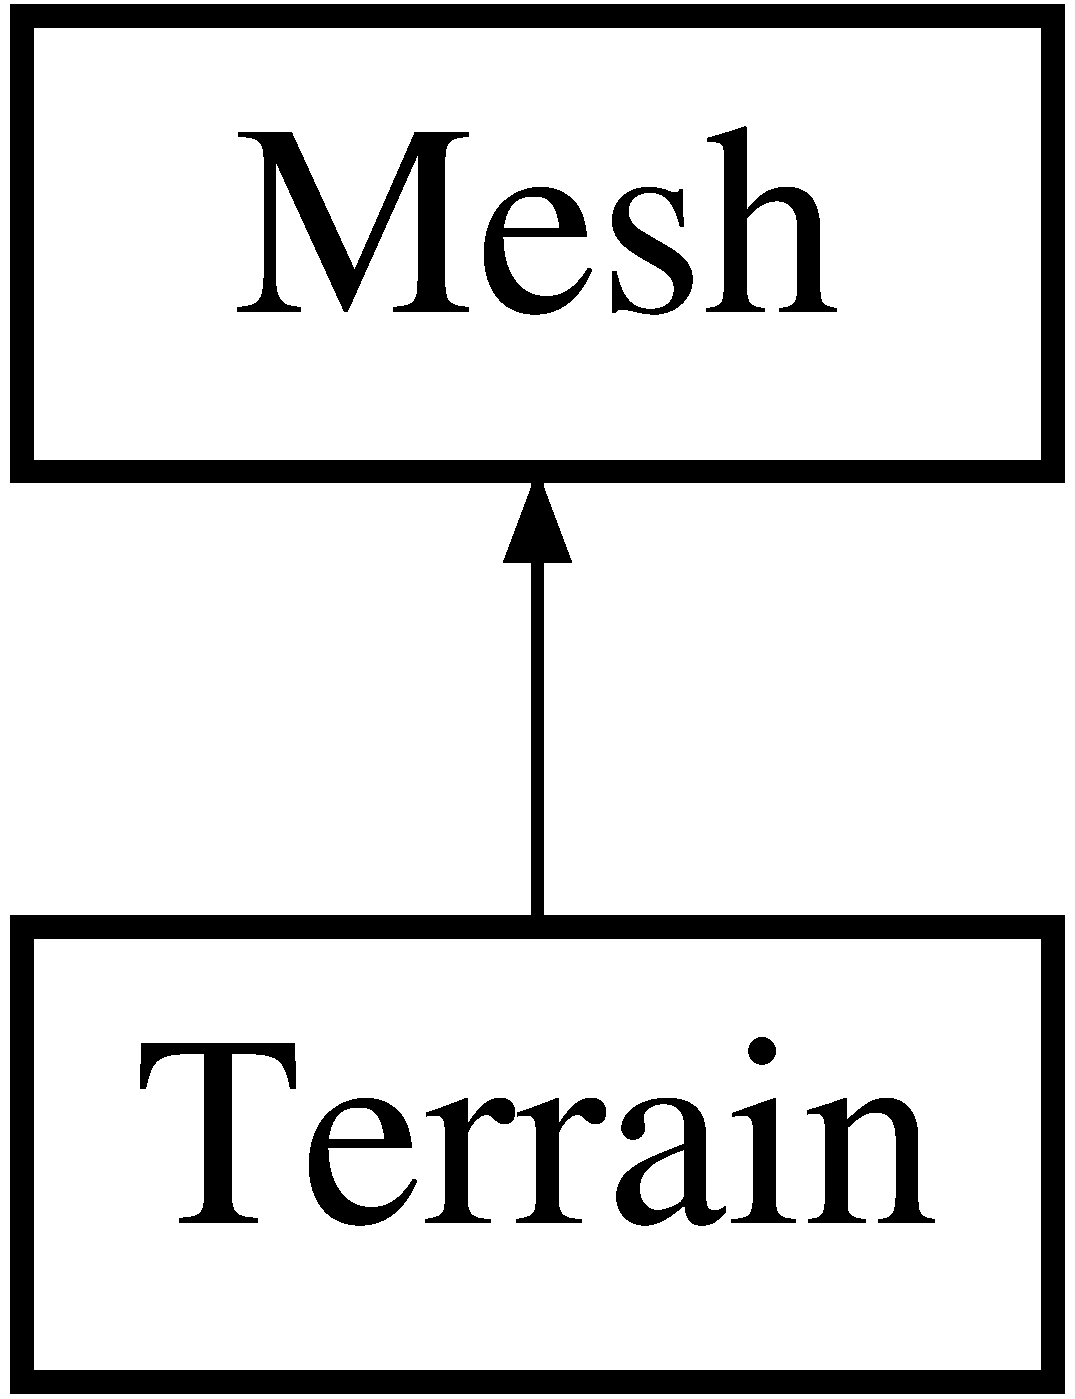
\includegraphics[height=2.000000cm]{class_terrain}
\end{center}
\end{figure}
\subsection*{Fonctions membres publiques}
\begin{DoxyCompactItemize}
\item 
\hyperlink{class_terrain_acebfe49e26563a8c2ca49e44a74fb40f}{Terrain} (float \hyperlink{class_terrain_ae25fe0ac0800f0e1c57c9b33f38f5a37}{longueur}, float \hyperlink{class_terrain_a1153a4642fd691e7fe25f9af1faba132}{largeur})
\begin{DoxyCompactList}\small\item\em Constructeur de \hyperlink{class_terrain_noise}{Terrain\+Noise}. \end{DoxyCompactList}\item 
\hyperlink{class_terrain_aeae81c7f546cae03d468363b558f5beb}{Terrain} (float \hyperlink{class_terrain_ae25fe0ac0800f0e1c57c9b33f38f5a37}{longueur}, float \hyperlink{class_terrain_a1153a4642fd691e7fe25f9af1faba132}{largeur}, float amplitude)
\begin{DoxyCompactList}\small\item\em Constructeur de \hyperlink{class_terrain_noise}{Terrain\+Noise}. \end{DoxyCompactList}\item 
float \hyperlink{class_terrain_a8892842d80a9737a1aabd9505a0fb49f}{get\+Hauteur} (float x, float y) const 
\begin{DoxyCompactList}\small\item\em Détermine la hauteur du terrain à la position {\itshape x}, {\itshape y}. ~\newline
Regarde si la position est sur ou en dehors du terrain. ~\newline
Passe le relai à \hyperlink{class_terrain_a63c855275f8270ccc0203bde0776a08f}{get\+Hauteur\+X\+Y()}. \end{DoxyCompactList}\item 
float \hyperlink{class_terrain_aadd802c62f67a5cfbbf820d31b45f87c}{get\+Hauteur} (const Vector2f \&point\+X\+Y) const 
\begin{DoxyCompactList}\small\item\em Surchage de la methode get\+Hauteur(float x, float y). \end{DoxyCompactList}\item 
float \hyperlink{class_terrain_a53105ed5f4b2dceadf432b52c7dbb5a3}{get\+Hauteur} (const Vector3f \&point\+X\+Y\+Z) const 
\begin{DoxyCompactList}\small\item\em Surchage de la methode get\+Hauteur(const Vector2f\& point\+X\+Y). \end{DoxyCompactList}\item 
void \hyperlink{class_terrain_a0a1bdaf1c083c94f8abb0cf28c14ae94}{get\+Color} (float \&r, float \&g, float \&b, float x, float y) const 
\begin{DoxyCompactList}\small\item\em Détermine la couleur de texture suivant une hauteur. \end{DoxyCompactList}\item 
bool \hyperlink{class_terrain_a732fa3071315926ba8f65f2fdf3acd23}{intersect} (const \hyperlink{class_rayon}{Rayon} \&rayon, float \&coeff\+Distance, int \&i) const 
\begin{DoxyCompactList}\small\item\em Test si un rayon traverse le terrain. ~\newline
Si c\textquotesingle{}est le cas, la methode retournera la distance d\textquotesingle{}intersection la plus proche sur le terrain. (cf. \hyperlink{class_rayon}{Rayon}) ~\newline
Utilise la méthode \hyperlink{class_terrain_a732fa3071315926ba8f65f2fdf3acd23}{intersect()} de \hyperlink{class_box}{Box}. \end{DoxyCompactList}\item 
\hypertarget{class_terrain_a50ed0e99f87cf87404c32c437cc6e20f}{}float {\bfseries get\+Min\+Elevation} () const \label{class_terrain_a50ed0e99f87cf87404c32c437cc6e20f}

\item 
\hypertarget{class_terrain_af50861f0e70b46e4bead8714f9e00c03}{}float {\bfseries get\+Max\+Elevation} () const \label{class_terrain_af50861f0e70b46e4bead8714f9e00c03}

\item 
Eigen\+::\+Vector3f \hyperlink{class_terrain_a60758bba8c5f1cfefe60498dab2b571d}{get\+Normal} (float x, float y) const 
\begin{DoxyCompactList}\small\item\em Détermine la normal du terrain à la position {\itshape x}, {\itshape y}. ~\newline
Regarde si les positions sont sur ou en dehors du terrain. ~\newline
Passe le relai à \hyperlink{class_terrain_a8b666ed9d5f948734b0d1c49adb6b535}{get\+Normal\+X\+Y()}. \end{DoxyCompactList}\item 
Eigen\+::\+Vector3f \hyperlink{class_terrain_a7c232e0d5b97f497e37229c8927dc112}{get\+Normal} (const Vector2f \&point\+X\+Y) const 
\begin{DoxyCompactList}\small\item\em Surchage de la methode get\+Normal(float x, float y). \end{DoxyCompactList}\item 
Eigen\+::\+Vector3f \hyperlink{class_terrain_a885582cef2dfe1133db04045725f73bd}{get\+Normal} (const Vector3f \&point\+X\+Y\+Z) const 
\begin{DoxyCompactList}\small\item\em Surchage de la methode get\+Hauteur(const Vector2f\& point\+X\+Y). \end{DoxyCompactList}\item 
bool \hyperlink{class_terrain_a75b8699997d2aff3eb461cf8a9220bb4}{in\+Out} (const Eigen\+::\+Vector3f \&point\+X\+Y\+Z) const 
\begin{DoxyCompactList}\small\item\em Test si le point {\itshape point\+X\+Y\+Z} est sous le terrain. \end{DoxyCompactList}\item 
virtual float \hyperlink{class_terrain_a63c855275f8270ccc0203bde0776a08f}{get\+Hauteur\+X\+Y} (float x, float y) const  =0
\begin{DoxyCompactList}\small\item\em Methode virtuel pour déterminer la hauteur du terrain à un point. ~\newline
A redéfinir dans les classes filles. (cf. \hyperlink{class_terrain_noise}{Terrain\+Noise} et \hyperlink{class_terrain_tab}{Terrain\+Tab}) \end{DoxyCompactList}\end{DoxyCompactItemize}
\subsection*{Attributs publics}
\begin{DoxyCompactItemize}
\item 
\hypertarget{class_terrain_ab31cb1bf848ab141c994897ee15858f5}{}\hyperlink{class_box}{Box} \hyperlink{class_terrain_ab31cb1bf848ab141c994897ee15858f5}{box}\label{class_terrain_ab31cb1bf848ab141c994897ee15858f5}

\begin{DoxyCompactList}\small\item\em La boite englobante du terrain. (cf. \hyperlink{class_box}{Box}) \end{DoxyCompactList}\item 
\hypertarget{class_terrain_ae25fe0ac0800f0e1c57c9b33f38f5a37}{}float \hyperlink{class_terrain_ae25fe0ac0800f0e1c57c9b33f38f5a37}{longueur}\label{class_terrain_ae25fe0ac0800f0e1c57c9b33f38f5a37}

\begin{DoxyCompactList}\small\item\em Distance du terrain en metre sur l\textquotesingle{}axe y. \end{DoxyCompactList}\item 
\hypertarget{class_terrain_a1153a4642fd691e7fe25f9af1faba132}{}float \hyperlink{class_terrain_a1153a4642fd691e7fe25f9af1faba132}{largeur}\label{class_terrain_a1153a4642fd691e7fe25f9af1faba132}

\begin{DoxyCompactList}\small\item\em Distance du terrain en metre sur l\textquotesingle{}axe x. \end{DoxyCompactList}\item 
\hypertarget{class_terrain_ab03b1edc97dc5d468eae0779bfcb805a}{}\hyperlink{class_color_gradient}{Color\+Gradient} \hyperlink{class_terrain_ab03b1edc97dc5d468eae0779bfcb805a}{heat\+Map\+Gradient}\label{class_terrain_ab03b1edc97dc5d468eae0779bfcb805a}

\begin{DoxyCompactList}\small\item\em Conteneur de tableau de couleur. (cf. \hyperlink{class_color_gradient}{Color\+Gradient}) \end{DoxyCompactList}\item 
\hypertarget{class_terrain_aad0e8c34a758f963efb3e4a89ba10cbc}{}float \hyperlink{class_terrain_aad0e8c34a758f963efb3e4a89ba10cbc}{hauteur\+Max}\label{class_terrain_aad0e8c34a758f963efb3e4a89ba10cbc}

\begin{DoxyCompactList}\small\item\em hauteur\+Max Altitude max du terrain. \end{DoxyCompactList}\item 
\hypertarget{class_terrain_ac89016fab6410586b08877b5c9790f27}{}float \hyperlink{class_terrain_ac89016fab6410586b08877b5c9790f27}{hauteur\+Min}\label{class_terrain_ac89016fab6410586b08877b5c9790f27}

\begin{DoxyCompactList}\small\item\em hauteur\+Min Altitude min du terrain. \end{DoxyCompactList}\end{DoxyCompactItemize}
\subsection*{Fonctions membres protégées}
\begin{DoxyCompactItemize}
\item 
virtual Eigen\+::\+Vector3f \hyperlink{class_terrain_a8b666ed9d5f948734b0d1c49adb6b535}{get\+Normal\+X\+Y} (float x, float y) const  =0
\begin{DoxyCompactList}\small\item\em Methode virtuel pour déterminer la normal du terrain à un point. ~\newline
. \end{DoxyCompactList}\item 
\hypertarget{class_terrain_a43f84c68d70b49af90637150c30e6f8b}{}void {\bfseries translate2} (const Vector3f \&t)\label{class_terrain_a43f84c68d70b49af90637150c30e6f8b}

\item 
\hypertarget{class_terrain_a9d8a4b5fabf8b8840a623ddf070cd866}{}virtual float {\bfseries min\+Elevation} () const  =0\label{class_terrain_a9d8a4b5fabf8b8840a623ddf070cd866}

\item 
\hypertarget{class_terrain_abd5ed37d041486bb06e7fedd5fa964a4}{}virtual float {\bfseries max\+Elevation} () const  =0\label{class_terrain_abd5ed37d041486bb06e7fedd5fa964a4}

\end{DoxyCompactItemize}


\subsection{Description détaillée}
Classe virtuelle de terrain. Sert de modèle pour les classes files \hyperlink{class_terrain_noise}{Terrain\+Noise} et \hyperlink{class_terrain_tab}{Terrain\+Tab}. 

\subsection{Documentation des constructeurs et destructeur}
\hypertarget{class_terrain_acebfe49e26563a8c2ca49e44a74fb40f}{}\index{Terrain@{Terrain}!Terrain@{Terrain}}
\index{Terrain@{Terrain}!Terrain@{Terrain}}
\subsubsection[{Terrain(float longueur, float largeur)}]{\setlength{\rightskip}{0pt plus 5cm}Terrain\+::\+Terrain (
\begin{DoxyParamCaption}
\item[{float}]{longueur, }
\item[{float}]{largeur}
\end{DoxyParamCaption}
)}\label{class_terrain_acebfe49e26563a8c2ca49e44a74fb40f}


Constructeur de \hyperlink{class_terrain_noise}{Terrain\+Noise}. 


\begin{DoxyParams}[1]{Paramètres}
\mbox{\tt in}  & {\em longueur} & Distance du terrain en metre sur l\textquotesingle{}axe y \\
\hline
\mbox{\tt in}  & {\em largeur} & Distance du terrain en metre sur l\textquotesingle{}axe x \\
\hline
\end{DoxyParams}
\hypertarget{class_terrain_aeae81c7f546cae03d468363b558f5beb}{}\index{Terrain@{Terrain}!Terrain@{Terrain}}
\index{Terrain@{Terrain}!Terrain@{Terrain}}
\subsubsection[{Terrain(float longueur, float largeur, float amplitude)}]{\setlength{\rightskip}{0pt plus 5cm}Terrain\+::\+Terrain (
\begin{DoxyParamCaption}
\item[{float}]{longueur, }
\item[{float}]{largeur, }
\item[{float}]{amplitude}
\end{DoxyParamCaption}
)}\label{class_terrain_aeae81c7f546cae03d468363b558f5beb}


Constructeur de \hyperlink{class_terrain_noise}{Terrain\+Noise}. 


\begin{DoxyParams}[1]{Paramètres}
\mbox{\tt in}  & {\em longueur} & Distance du terrain en metre sur l\textquotesingle{}axe y \\
\hline
\mbox{\tt in}  & {\em largeur} & Distance du terrain en metre sur l\textquotesingle{}axe x \\
\hline
\mbox{\tt in}  & {\em amplitude} & Amplitude Max que pourra atteindre la terrain. \\
\hline
\end{DoxyParams}


\subsection{Documentation des fonctions membres}
\hypertarget{class_terrain_a0a1bdaf1c083c94f8abb0cf28c14ae94}{}\index{Terrain@{Terrain}!get\+Color@{get\+Color}}
\index{get\+Color@{get\+Color}!Terrain@{Terrain}}
\subsubsection[{get\+Color(float \&r, float \&g, float \&b, float x, float y) const }]{\setlength{\rightskip}{0pt plus 5cm}void Terrain\+::get\+Color (
\begin{DoxyParamCaption}
\item[{float \&}]{r, }
\item[{float \&}]{g, }
\item[{float \&}]{b, }
\item[{float}]{x, }
\item[{float}]{y}
\end{DoxyParamCaption}
) const}\label{class_terrain_a0a1bdaf1c083c94f8abb0cf28c14ae94}


Détermine la couleur de texture suivant une hauteur. 


\begin{DoxyParams}[1]{Paramètres}
\mbox{\tt out}  & {\em r} & La valeur rouge de la couleur. \\
\hline
\mbox{\tt out}  & {\em g} & La valeur vert de la couleur. \\
\hline
\mbox{\tt out}  & {\em b} & La valeur bleu de la couleur. \\
\hline
\mbox{\tt in}  & {\em x} & Position en {\itshape x} du point de couleur à déterminer. \\
\hline
\mbox{\tt in}  & {\em y} & Position en {\itshape y} du point de couleur à déterminer. \\
\hline
\end{DoxyParams}
\hypertarget{class_terrain_a8892842d80a9737a1aabd9505a0fb49f}{}\index{Terrain@{Terrain}!get\+Hauteur@{get\+Hauteur}}
\index{get\+Hauteur@{get\+Hauteur}!Terrain@{Terrain}}
\subsubsection[{get\+Hauteur(float x, float y) const }]{\setlength{\rightskip}{0pt plus 5cm}float Terrain\+::get\+Hauteur (
\begin{DoxyParamCaption}
\item[{float}]{x, }
\item[{float}]{y}
\end{DoxyParamCaption}
) const}\label{class_terrain_a8892842d80a9737a1aabd9505a0fb49f}


Détermine la hauteur du terrain à la position {\itshape x}, {\itshape y}. ~\newline
Regarde si la position est sur ou en dehors du terrain. ~\newline
Passe le relai à \hyperlink{class_terrain_a63c855275f8270ccc0203bde0776a08f}{get\+Hauteur\+X\+Y()}. 


\begin{DoxyParams}[1]{Paramètres}
\mbox{\tt in}  & {\em x} & position en {\itshape x} de la hauteur à déterminer. \\
\hline
\mbox{\tt in}  & {\em y} & position en {\itshape y} de la hauteur à déterminer. \\
\hline
\end{DoxyParams}
\begin{DoxyReturn}{Renvoie}
la hauteur du terrain à la position {\itshape x}, {\itshape y}. Si la position est hors map, la valeur sera H\+A\+U\+T\+E\+U\+R\+\_\+\+H\+O\+R\+S\+\_\+\+M\+A\+P. 
\end{DoxyReturn}
\hypertarget{class_terrain_aadd802c62f67a5cfbbf820d31b45f87c}{}\index{Terrain@{Terrain}!get\+Hauteur@{get\+Hauteur}}
\index{get\+Hauteur@{get\+Hauteur}!Terrain@{Terrain}}
\subsubsection[{get\+Hauteur(const Vector2f \&point\+X\+Y) const }]{\setlength{\rightskip}{0pt plus 5cm}float Terrain\+::get\+Hauteur (
\begin{DoxyParamCaption}
\item[{const Vector2f \&}]{point\+X\+Y}
\end{DoxyParamCaption}
) const}\label{class_terrain_aadd802c62f67a5cfbbf820d31b45f87c}


Surchage de la methode get\+Hauteur(float x, float y). 


\begin{DoxyParams}[1]{Paramètres}
\mbox{\tt in}  & {\em point\+X\+Y} & Un point comprenant uniquement les axes {\itshape x}, {\itshape y}. \\
\hline
\end{DoxyParams}
\begin{DoxyReturn}{Renvoie}
la hauteur du terrain au point {\itshape point\+X\+Y}. 
\end{DoxyReturn}
\hypertarget{class_terrain_a53105ed5f4b2dceadf432b52c7dbb5a3}{}\index{Terrain@{Terrain}!get\+Hauteur@{get\+Hauteur}}
\index{get\+Hauteur@{get\+Hauteur}!Terrain@{Terrain}}
\subsubsection[{get\+Hauteur(const Vector3f \&point\+X\+Y\+Z) const }]{\setlength{\rightskip}{0pt plus 5cm}float Terrain\+::get\+Hauteur (
\begin{DoxyParamCaption}
\item[{const Vector3f \&}]{point\+X\+Y\+Z}
\end{DoxyParamCaption}
) const}\label{class_terrain_a53105ed5f4b2dceadf432b52c7dbb5a3}


Surchage de la methode get\+Hauteur(const Vector2f\& point\+X\+Y). 


\begin{DoxyParams}[1]{Paramètres}
\mbox{\tt in}  & {\em point\+X\+Y\+Z} & Un point comprenant uniquement les axes {\itshape x}, {\itshape y}, {\itshape z}. \\
\hline
\end{DoxyParams}
\begin{DoxyReturn}{Renvoie}
la hauteur du terrain au point {\itshape point\+X\+Y\+Z}. 
\end{DoxyReturn}
\hypertarget{class_terrain_a63c855275f8270ccc0203bde0776a08f}{}\index{Terrain@{Terrain}!get\+Hauteur\+X\+Y@{get\+Hauteur\+X\+Y}}
\index{get\+Hauteur\+X\+Y@{get\+Hauteur\+X\+Y}!Terrain@{Terrain}}
\subsubsection[{get\+Hauteur\+X\+Y(float x, float y) const  =0}]{\setlength{\rightskip}{0pt plus 5cm}virtual float Terrain\+::get\+Hauteur\+X\+Y (
\begin{DoxyParamCaption}
\item[{float}]{x, }
\item[{float}]{y}
\end{DoxyParamCaption}
) const\hspace{0.3cm}{\ttfamily [pure virtual]}}\label{class_terrain_a63c855275f8270ccc0203bde0776a08f}


Methode virtuel pour déterminer la hauteur du terrain à un point. ~\newline
A redéfinir dans les classes filles. (cf. \hyperlink{class_terrain_noise}{Terrain\+Noise} et \hyperlink{class_terrain_tab}{Terrain\+Tab}) 


\begin{DoxyParams}[1]{Paramètres}
\mbox{\tt in}  & {\em x} & la position en x du point. \\
\hline
\mbox{\tt in}  & {\em y} & la position en y du point. \\
\hline
\end{DoxyParams}
\begin{DoxyReturn}{Renvoie}
la hauteur du terrain au point donné. 
\end{DoxyReturn}


Implémenté dans \hyperlink{class_terrain_tab_a076546e6958b6b2edd94366976e21c78}{Terrain\+Tab}, et \hyperlink{class_terrain_noise_a4173f17958ed358f9b4a6b005b0ed256}{Terrain\+Noise}.

\hypertarget{class_terrain_a60758bba8c5f1cfefe60498dab2b571d}{}\index{Terrain@{Terrain}!get\+Normal@{get\+Normal}}
\index{get\+Normal@{get\+Normal}!Terrain@{Terrain}}
\subsubsection[{get\+Normal(float x, float y) const }]{\setlength{\rightskip}{0pt plus 5cm}Vector3f Terrain\+::get\+Normal (
\begin{DoxyParamCaption}
\item[{float}]{x, }
\item[{float}]{y}
\end{DoxyParamCaption}
) const}\label{class_terrain_a60758bba8c5f1cfefe60498dab2b571d}


Détermine la normal du terrain à la position {\itshape x}, {\itshape y}. ~\newline
Regarde si les positions sont sur ou en dehors du terrain. ~\newline
Passe le relai à \hyperlink{class_terrain_a8b666ed9d5f948734b0d1c49adb6b535}{get\+Normal\+X\+Y()}. 


\begin{DoxyParams}[1]{Paramètres}
\mbox{\tt in}  & {\em x} & position en {\itshape x} de la normal à déterminer. \\
\hline
\mbox{\tt in}  & {\em y} & position en {\itshape y} de la normal à déterminer. \\
\hline
\end{DoxyParams}
\begin{DoxyReturn}{Renvoie}
la hauteur du terrain à la position {\itshape x}, {\itshape y}. Si la position est hors map, la valeur sera un vecteur nul. 
\end{DoxyReturn}
\hypertarget{class_terrain_a7c232e0d5b97f497e37229c8927dc112}{}\index{Terrain@{Terrain}!get\+Normal@{get\+Normal}}
\index{get\+Normal@{get\+Normal}!Terrain@{Terrain}}
\subsubsection[{get\+Normal(const Vector2f \&point\+X\+Y) const }]{\setlength{\rightskip}{0pt plus 5cm}Vector3f Terrain\+::get\+Normal (
\begin{DoxyParamCaption}
\item[{const Vector2f \&}]{point\+X\+Y}
\end{DoxyParamCaption}
) const}\label{class_terrain_a7c232e0d5b97f497e37229c8927dc112}


Surchage de la methode get\+Normal(float x, float y). 


\begin{DoxyParams}[1]{Paramètres}
\mbox{\tt in}  & {\em point\+X\+Y} & Un point comprenant uniquement les axes {\itshape x}, {\itshape y}. \\
\hline
\end{DoxyParams}
\begin{DoxyReturn}{Renvoie}
la normal du terrain au point {\itshape point\+X\+Y}. 
\end{DoxyReturn}
\hypertarget{class_terrain_a885582cef2dfe1133db04045725f73bd}{}\index{Terrain@{Terrain}!get\+Normal@{get\+Normal}}
\index{get\+Normal@{get\+Normal}!Terrain@{Terrain}}
\subsubsection[{get\+Normal(const Vector3f \&point\+X\+Y\+Z) const }]{\setlength{\rightskip}{0pt plus 5cm}Vector3f Terrain\+::get\+Normal (
\begin{DoxyParamCaption}
\item[{const Vector3f \&}]{point\+X\+Y\+Z}
\end{DoxyParamCaption}
) const}\label{class_terrain_a885582cef2dfe1133db04045725f73bd}


Surchage de la methode get\+Hauteur(const Vector2f\& point\+X\+Y). 


\begin{DoxyParams}[1]{Paramètres}
\mbox{\tt in}  & {\em point\+X\+Y\+Z} & Un point comprenant uniquement les axes {\itshape x}, {\itshape y}, {\itshape z}. \\
\hline
\end{DoxyParams}
\begin{DoxyReturn}{Renvoie}
la normal du terrain au point {\itshape point\+X\+Y\+Z}. 
\end{DoxyReturn}
\hypertarget{class_terrain_a8b666ed9d5f948734b0d1c49adb6b535}{}\index{Terrain@{Terrain}!get\+Normal\+X\+Y@{get\+Normal\+X\+Y}}
\index{get\+Normal\+X\+Y@{get\+Normal\+X\+Y}!Terrain@{Terrain}}
\subsubsection[{get\+Normal\+X\+Y(float x, float y) const  =0}]{\setlength{\rightskip}{0pt plus 5cm}virtual Eigen\+::\+Vector3f Terrain\+::get\+Normal\+X\+Y (
\begin{DoxyParamCaption}
\item[{float}]{x, }
\item[{float}]{y}
\end{DoxyParamCaption}
) const\hspace{0.3cm}{\ttfamily [protected]}, {\ttfamily [pure virtual]}}\label{class_terrain_a8b666ed9d5f948734b0d1c49adb6b535}


Methode virtuel pour déterminer la normal du terrain à un point. ~\newline
. 


\begin{DoxyParams}[1]{Paramètres}
\mbox{\tt in}  & {\em x} & la position en x du point. \\
\hline
\mbox{\tt in}  & {\em y} & la position en y du point. \\
\hline
\end{DoxyParams}
\begin{DoxyReturn}{Renvoie}
La normale à la position {\itshape x},{\itshape y}. 
\end{DoxyReturn}


Implémenté dans \hyperlink{class_terrain_tab_aaf94ed8b78c53bb798f7879c9249f3b3}{Terrain\+Tab}, et \hyperlink{class_terrain_noise_af50426bd1451cec938411d6bb5f82ac0}{Terrain\+Noise}.

\hypertarget{class_terrain_a75b8699997d2aff3eb461cf8a9220bb4}{}\index{Terrain@{Terrain}!in\+Out@{in\+Out}}
\index{in\+Out@{in\+Out}!Terrain@{Terrain}}
\subsubsection[{in\+Out(const Eigen\+::\+Vector3f \&point\+X\+Y\+Z) const }]{\setlength{\rightskip}{0pt plus 5cm}bool Terrain\+::in\+Out (
\begin{DoxyParamCaption}
\item[{const Eigen\+::\+Vector3f \&}]{point\+X\+Y\+Z}
\end{DoxyParamCaption}
) const}\label{class_terrain_a75b8699997d2aff3eb461cf8a9220bb4}


Test si le point {\itshape point\+X\+Y\+Z} est sous le terrain. 


\begin{DoxyParams}[1]{Paramètres}
\mbox{\tt in}  & {\em point\+X\+Y\+Z} & un point quelconque. \\
\hline
\end{DoxyParams}
\begin{DoxyReturn}{Renvoie}
Le resultat du test. Si le point point\+X\+Y\+Z est en dehors de la carte, la valeur sera false. 
\end{DoxyReturn}
\hypertarget{class_terrain_a732fa3071315926ba8f65f2fdf3acd23}{}\index{Terrain@{Terrain}!intersect@{intersect}}
\index{intersect@{intersect}!Terrain@{Terrain}}
\subsubsection[{intersect(const Rayon \&rayon, float \&coeff\+Distance, int \&i) const }]{\setlength{\rightskip}{0pt plus 5cm}bool Terrain\+::intersect (
\begin{DoxyParamCaption}
\item[{const {\bf Rayon} \&}]{rayon, }
\item[{float \&}]{coeff\+Distance, }
\item[{int \&}]{i}
\end{DoxyParamCaption}
) const}\label{class_terrain_a732fa3071315926ba8f65f2fdf3acd23}


Test si un rayon traverse le terrain. ~\newline
Si c\textquotesingle{}est le cas, la methode retournera la distance d\textquotesingle{}intersection la plus proche sur le terrain. (cf. \hyperlink{class_rayon}{Rayon}) ~\newline
Utilise la méthode \hyperlink{class_terrain_a732fa3071315926ba8f65f2fdf3acd23}{intersect()} de \hyperlink{class_box}{Box}. 


\begin{DoxyParams}[1]{Paramètres}
\mbox{\tt in}  & {\em rayon} & Un rayon quelconque. (cf. \hyperlink{class_rayon}{Rayon}) \\
\hline
\mbox{\tt out}  & {\em coeff\+Distance} & coefficient de distance de l\textquotesingle{}impacte sur le terrain par rapport à l\textquotesingle{}origine du rayon. ~\newline
Le coefficient est dependant de la norme du vecteur direction du rayon. \\
\hline
\mbox{\tt out}  & {\em Nombre} & d\textquotesingle{}itération durant le ray marching. \\
\hline
\end{DoxyParams}
\begin{DoxyReturn}{Renvoie}
Le resultat du test. True = intersection, false = pas d\textquotesingle{}intersection. 
\end{DoxyReturn}


La documentation de cette classe a été générée à partir des fichiers suivants \+:\begin{DoxyCompactItemize}
\item 
terrain/terrain.\+h\item 
terrain/terrain.\+cpp\end{DoxyCompactItemize}

\hypertarget{class_terrain_noise}{}\section{Référence de la classe Terrain\+Noise}
\label{class_terrain_noise}\index{Terrain\+Noise@{Terrain\+Noise}}


Classe fille de \hyperlink{class_terrain2}{Terrain2}. Elle s\textquotesingle{}appuis sur l\textquotesingle{}utilisation de noise pour déterminer la forme du terrain.  




{\ttfamily \#include $<$terrainnoise.\+h$>$}

Graphe d\textquotesingle{}héritage de Terrain\+Noise\+:\begin{figure}[H]
\begin{center}
\leavevmode
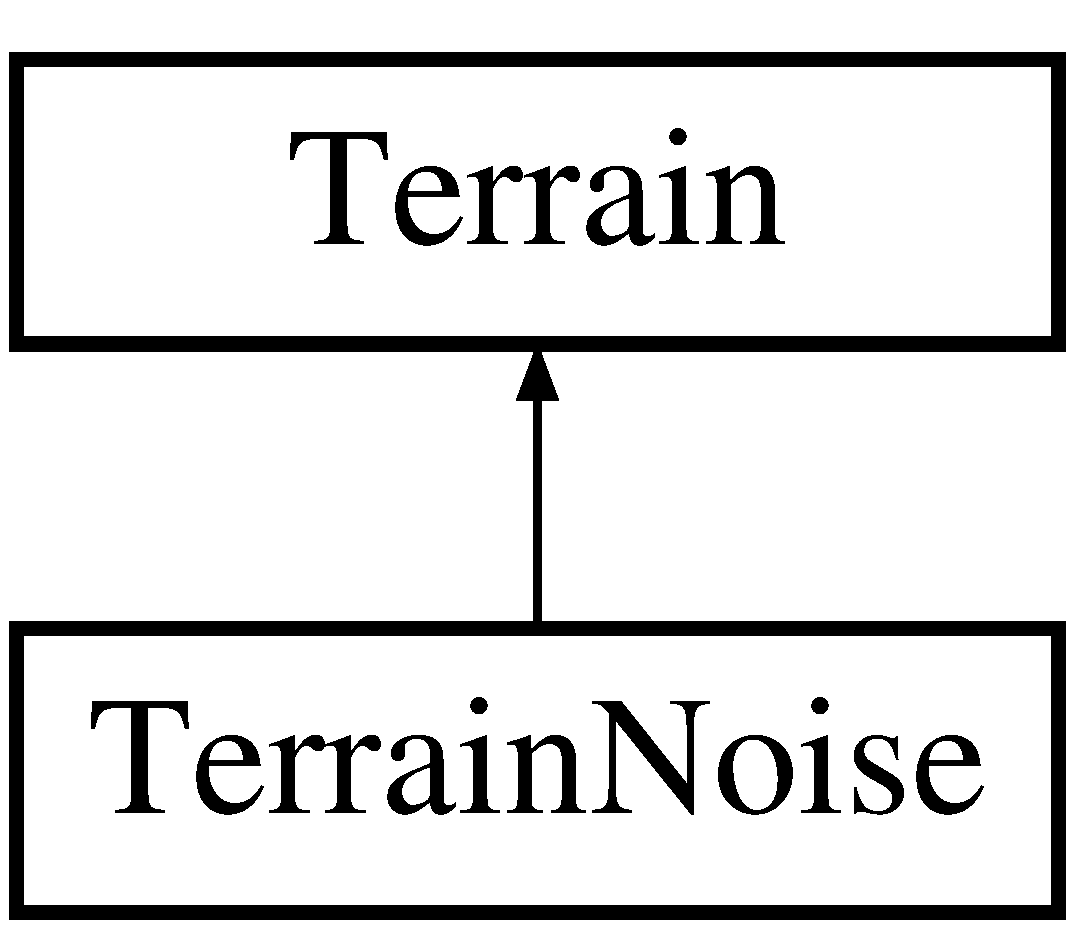
\includegraphics[height=3.000000cm]{class_terrain_noise}
\end{center}
\end{figure}
\subsection*{Fonctions membres publiques}
\begin{DoxyCompactItemize}
\item 
\hypertarget{class_terrain_noise_ade7285caeec8d121790159ad6b0af25f}{}{\bfseries Terrain\+Noise} (int \+\_\+longueur, int \+\_\+largeur)\label{class_terrain_noise_ade7285caeec8d121790159ad6b0af25f}

\end{DoxyCompactItemize}
\subsection*{Fonctions membres protégées}
\begin{DoxyCompactItemize}
\item 
float \hyperlink{class_terrain_noise_a4173f17958ed358f9b4a6b005b0ed256}{get\+Hauteur\+X\+Y} (float x, float y) const 
\begin{DoxyCompactList}\small\item\em Récupere la hauteur du terrain à un point donné. \end{DoxyCompactList}\item 
float \hyperlink{class_terrain_noise_aa22eddb4730bc005cebc2d6d62c437d6}{noise} (int amplitude, float periode, float x, float y) const 
\begin{DoxyCompactList}\small\item\em Récupération d\textquotesingle{}une valeur de noise suivant les paramétres donnés. \end{DoxyCompactList}\item 
float \hyperlink{class_terrain_noise_ad3dc579820ae6931c246406f55bbe5b0}{ridge} (float hauteur, float seuil) const 
\begin{DoxyCompactList}\small\item\em Application sur une valeur de hauteur d\textquotesingle{}un ridge (seuil avec rebond) suivant un seuil. \end{DoxyCompactList}\end{DoxyCompactItemize}
\subsection*{Membres hérités additionnels}


\subsection{Description détaillée}
Classe fille de \hyperlink{class_terrain2}{Terrain2}. Elle s\textquotesingle{}appuis sur l\textquotesingle{}utilisation de noise pour déterminer la forme du terrain. 

\subsection{Documentation des fonctions membres}
\hypertarget{class_terrain_noise_a4173f17958ed358f9b4a6b005b0ed256}{}\index{Terrain\+Noise@{Terrain\+Noise}!get\+Hauteur\+X\+Y@{get\+Hauteur\+X\+Y}}
\index{get\+Hauteur\+X\+Y@{get\+Hauteur\+X\+Y}!Terrain\+Noise@{Terrain\+Noise}}
\subsubsection[{get\+Hauteur\+X\+Y(float x, float y) const }]{\setlength{\rightskip}{0pt plus 5cm}float Terrain\+Noise\+::get\+Hauteur\+X\+Y (
\begin{DoxyParamCaption}
\item[{float}]{x, }
\item[{float}]{y}
\end{DoxyParamCaption}
) const\hspace{0.3cm}{\ttfamily [protected]}, {\ttfamily [virtual]}}\label{class_terrain_noise_a4173f17958ed358f9b4a6b005b0ed256}


Récupere la hauteur du terrain à un point donné. 


\begin{DoxyParams}{Paramètres}
{\em x} & la position en x du point. \\
\hline
{\em y} & la position en y du point. \\
\hline
\end{DoxyParams}
\begin{DoxyReturn}{Renvoie}
la hauteur du terrain au point donné. 
\end{DoxyReturn}


Implémente \hyperlink{class_terrain2}{Terrain2}.

\hypertarget{class_terrain_noise_aa22eddb4730bc005cebc2d6d62c437d6}{}\index{Terrain\+Noise@{Terrain\+Noise}!noise@{noise}}
\index{noise@{noise}!Terrain\+Noise@{Terrain\+Noise}}
\subsubsection[{noise(int amplitude, float periode, float x, float y) const }]{\setlength{\rightskip}{0pt plus 5cm}float Terrain\+Noise\+::noise (
\begin{DoxyParamCaption}
\item[{int}]{amplitude, }
\item[{float}]{periode, }
\item[{float}]{x, }
\item[{float}]{y}
\end{DoxyParamCaption}
) const\hspace{0.3cm}{\ttfamily [protected]}}\label{class_terrain_noise_aa22eddb4730bc005cebc2d6d62c437d6}


Récupération d\textquotesingle{}une valeur de noise suivant les paramétres donnés. 


\begin{DoxyParams}{Paramètres}
{\em amplitude} & Amplitude max que pourra atteindre le noise. \\
\hline
{\em periode} & Distance en metre pour que le noise atteigne un cycle. \\
\hline
{\em x} & Position en x d\textquotesingle{}un point donné au noise. \\
\hline
{\em y} & Position en y d\textquotesingle{}un point donné au noise. \\
\hline
\end{DoxyParams}
\begin{DoxyReturn}{Renvoie}
La valeur générée par le noise. 
\end{DoxyReturn}
\hypertarget{class_terrain_noise_ad3dc579820ae6931c246406f55bbe5b0}{}\index{Terrain\+Noise@{Terrain\+Noise}!ridge@{ridge}}
\index{ridge@{ridge}!Terrain\+Noise@{Terrain\+Noise}}
\subsubsection[{ridge(float hauteur, float seuil) const }]{\setlength{\rightskip}{0pt plus 5cm}float Terrain\+Noise\+::ridge (
\begin{DoxyParamCaption}
\item[{float}]{hauteur, }
\item[{float}]{seuil}
\end{DoxyParamCaption}
) const\hspace{0.3cm}{\ttfamily [protected]}}\label{class_terrain_noise_ad3dc579820ae6931c246406f55bbe5b0}


Application sur une valeur de hauteur d\textquotesingle{}un ridge (seuil avec rebond) suivant un seuil. 


\begin{DoxyParams}{Paramètres}
{\em hauteur} & La hauteur à soumettre au ridge. \\
\hline
{\em seuil} & Le seuil d\textquotesingle{}application du ridge. Si le seuil est au-\/dessus du maximum atteignable par la hauteur, aucun ridge ne pourra être appliqué dessus. \\
\hline
\end{DoxyParams}
\begin{DoxyReturn}{Renvoie}
La hauteur après avoir passé le ridge. 
\end{DoxyReturn}


La documentation de cette classe a été générée à partir des fichiers suivants \+:\begin{DoxyCompactItemize}
\item 
terrain/terrainnoise.\+h\item 
terrain/terrainnoise.\+cpp\end{DoxyCompactItemize}

\hypertarget{class_terrain_tab}{}\section{Référence de la classe Terrain\+Tab}
\label{class_terrain_tab}\index{Terrain\+Tab@{Terrain\+Tab}}


Classe fille de \hyperlink{class_terrain}{Terrain}. Elle s\textquotesingle{}appuis sur l\textquotesingle{}utilisation d\textquotesingle{}un image High\+Map pour déterminer la forme du terrain.  




{\ttfamily \#include $<$terraintab.\+h$>$}

Graphe d\textquotesingle{}héritage de Terrain\+Tab\+:\begin{figure}[H]
\begin{center}
\leavevmode
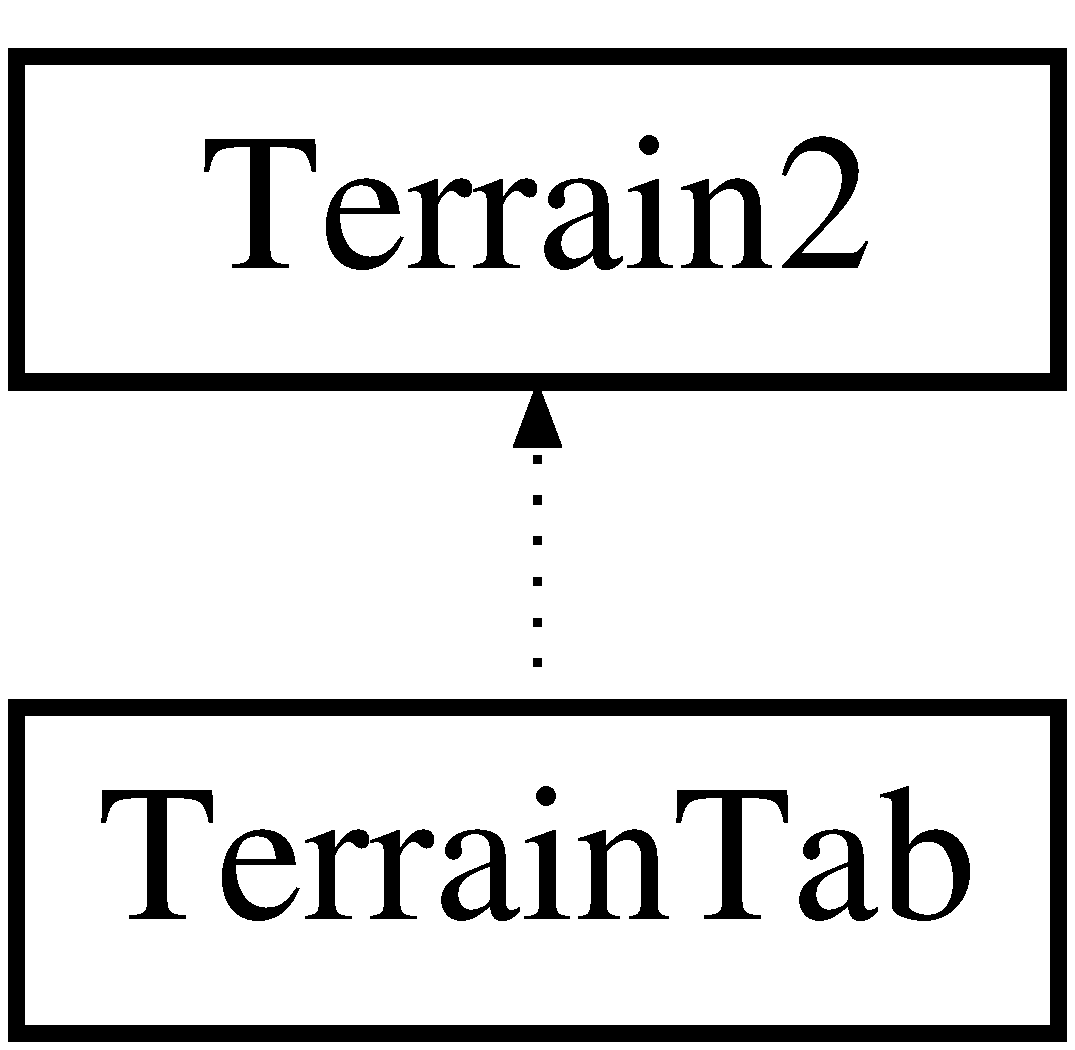
\includegraphics[height=2.000000cm]{class_terrain_tab}
\end{center}
\end{figure}
\subsection*{Fonctions membres publiques}
\begin{DoxyCompactItemize}
\item 
\hyperlink{class_terrain_tab_ac31e7a1fb2f33a2875de3353c3eba76a}{Terrain\+Tab} (const Q\+Image \&img, float \hyperlink{class_terrain_ae25fe0ac0800f0e1c57c9b33f38f5a37}{longueur}, float \hyperlink{class_terrain_a1153a4642fd691e7fe25f9af1faba132}{largeur}, float \hyperlink{class_terrain_tab_a46e3284a38c404d326323091628abf03}{amplitude}=1.\+0f)
\item 
\hyperlink{class_terrain_tab_a04adc95147a7eceeac2eda0a62aa971a}{Terrain\+Tab} (const Q\+Image \&img, int \+\_\+nb\+Height, int \+\_\+nb\+Width, float \hyperlink{class_terrain_ae25fe0ac0800f0e1c57c9b33f38f5a37}{longueur}, float \hyperlink{class_terrain_a1153a4642fd691e7fe25f9af1faba132}{largeur}, float \+\_\+amplitude=1.\+0f)
\item 
\hyperlink{class_terrain_tab_afb333a647c91855ed76c41cba60903f7}{Terrain\+Tab} (const \hyperlink{class_terrain_tab}{Terrain\+Tab} \&copy)
\begin{DoxyCompactList}\small\item\em Constructeur par copie. \end{DoxyCompactList}\end{DoxyCompactItemize}
\subsection*{Fonctions membres privées}
\begin{DoxyCompactItemize}
\item 
float \hyperlink{class_terrain_tab_a076546e6958b6b2edd94366976e21c78}{get\+Hauteur\+X\+Y} (float x, float y) const 
\begin{DoxyCompactList}\small\item\em Récupere la hauteur du terrain à un point donné. ~\newline
Redéfinition de la methode. (cf. \hyperlink{class_terrain}{Terrain}) \end{DoxyCompactList}\item 
Eigen\+::\+Vector3f \hyperlink{class_terrain_tab_aaf94ed8b78c53bb798f7879c9249f3b3}{get\+Normal\+X\+Y} (float x, float y) const 
\begin{DoxyCompactList}\small\item\em Calcul la normale d\textquotesingle{}un point sur le terrain. \end{DoxyCompactList}\item 
\hypertarget{class_terrain_tab_a6d4a9f721bcea94798b66d24a6ce065f}{}void \hyperlink{class_terrain_tab_a6d4a9f721bcea94798b66d24a6ce065f}{init\+Grille} ()\label{class_terrain_tab_a6d4a9f721bcea94798b66d24a6ce065f}

\begin{DoxyCompactList}\small\item\em Initialise et remplis la grille topographique avec l\textquotesingle{}image donnée dans le constructeur. Deplus les indications complémentaire \+: \+\_\+nb\+Height et \+\_\+nb\+Width sont utilisées dans le processus. \end{DoxyCompactList}\item 
void \hyperlink{class_terrain_tab_a1e83068235cd90e879667fc3c1b6c8d0}{simple\+Init\+Image} (const Q\+Image \&img)
\begin{DoxyCompactList}\small\item\em Initialise et remplis la grille topographique suivant l\textquotesingle{}image données en paramètre. La grille aura le même precision que l\textquotesingle{}image donnée. \end{DoxyCompactList}\item 
float \hyperlink{class_terrain_tab_ac004fb257c99905c71303d819c9b8df7}{get} (int x, int y) const 
\begin{DoxyCompactList}\small\item\em Récupere la hauteur du terrain à un point donné. Le point doit correspondre à un point existant sur la carte. Aucun approximation ne sera faite. \end{DoxyCompactList}\item 
\hypertarget{class_terrain_tab_a1e534af1daceb931f558245d8b584084}{}void \hyperlink{class_terrain_tab_a1e534af1daceb931f558245d8b584084}{update\+Min\+Elevation} ()\label{class_terrain_tab_a1e534af1daceb931f558245d8b584084}

\begin{DoxyCompactList}\small\item\em Détermine l\textquotesingle{}élévation minimum du terrain et ajuste \hyperlink{class_terrain_tab_ad8e9ca00da63f66915658151516d10fc}{hauteur\+Min}. \end{DoxyCompactList}\item 
\hypertarget{class_terrain_tab_a65271db7916caf5f8ebddf5aa1ad7021}{}void \hyperlink{class_terrain_tab_a65271db7916caf5f8ebddf5aa1ad7021}{update\+Max\+Elevation} ()\label{class_terrain_tab_a65271db7916caf5f8ebddf5aa1ad7021}

\begin{DoxyCompactList}\small\item\em Détermine l\textquotesingle{}élévation maximum du terrain et ajuste \hyperlink{class_terrain_tab_a6b8b4f7bd611b40d59e8b60e105ce1a8}{hauteur\+Max}. \end{DoxyCompactList}\item 
\hypertarget{class_terrain_tab_a09fcdcde6adeb9c3b51c1368380dbb6b}{}void \hyperlink{class_terrain_tab_a09fcdcde6adeb9c3b51c1368380dbb6b}{update\+Elevation} ()\label{class_terrain_tab_a09fcdcde6adeb9c3b51c1368380dbb6b}

\begin{DoxyCompactList}\small\item\em Détermine l\textquotesingle{}élévation minimum et maximum du terrain et ajuste \hyperlink{class_terrain_tab_ad8e9ca00da63f66915658151516d10fc}{hauteur\+Min}, \hyperlink{class_terrain_tab_a6b8b4f7bd611b40d59e8b60e105ce1a8}{hauteur\+Max}. \end{DoxyCompactList}\item 
float \hyperlink{class_terrain_tab_aa7bc7042c28393faf0813820ab1c1d6f}{min\+Elevation} () const 
\item 
float \hyperlink{class_terrain_tab_abbfa195b063129a3b96e6485cf37ad27}{max\+Elevation} () const 
\end{DoxyCompactItemize}
\subsection*{Attributs privés}
\begin{DoxyCompactItemize}
\item 
\hypertarget{class_terrain_tab_a8213ff78ba0bae26a3ca0391166a5128}{}int \hyperlink{class_terrain_tab_a8213ff78ba0bae26a3ca0391166a5128}{height}\label{class_terrain_tab_a8213ff78ba0bae26a3ca0391166a5128}

\begin{DoxyCompactList}\small\item\em height Hauteur de l\textquotesingle{}image High\+Map. \end{DoxyCompactList}\item 
\hypertarget{class_terrain_tab_a4cfde4817009ea768a1c071c00c2f1fd}{}int \hyperlink{class_terrain_tab_a4cfde4817009ea768a1c071c00c2f1fd}{width}\label{class_terrain_tab_a4cfde4817009ea768a1c071c00c2f1fd}

\begin{DoxyCompactList}\small\item\em width Largeur de l\textquotesingle{}image High\+Map. \end{DoxyCompactList}\item 
\hypertarget{class_terrain_tab_a46e3284a38c404d326323091628abf03}{}float \hyperlink{class_terrain_tab_a46e3284a38c404d326323091628abf03}{amplitude}\label{class_terrain_tab_a46e3284a38c404d326323091628abf03}

\begin{DoxyCompactList}\small\item\em amplitude Amplitude max attegnable par le terrain. \end{DoxyCompactList}\item 
\hypertarget{class_terrain_tab_a0b095b4aeb69aa00a75d543cd726e608}{}float $\ast$ \hyperlink{class_terrain_tab_a0b095b4aeb69aa00a75d543cd726e608}{grille} = nullptr\label{class_terrain_tab_a0b095b4aeb69aa00a75d543cd726e608}

\begin{DoxyCompactList}\small\item\em grille \end{DoxyCompactList}\item 
\hypertarget{class_terrain_tab_ace8f6807c917c7c186cf688e2c286f10}{}float $\ast$$\ast$ \hyperlink{class_terrain_tab_ace8f6807c917c7c186cf688e2c286f10}{grille2d} = nullptr\label{class_terrain_tab_ace8f6807c917c7c186cf688e2c286f10}

\begin{DoxyCompactList}\small\item\em grille2d \end{DoxyCompactList}\item 
\hypertarget{class_terrain_tab_a6b8b4f7bd611b40d59e8b60e105ce1a8}{}float \hyperlink{class_terrain_tab_a6b8b4f7bd611b40d59e8b60e105ce1a8}{hauteur\+Max}\label{class_terrain_tab_a6b8b4f7bd611b40d59e8b60e105ce1a8}

\begin{DoxyCompactList}\small\item\em hauteur\+Max Altitude max du terrain. \end{DoxyCompactList}\item 
\hypertarget{class_terrain_tab_ad8e9ca00da63f66915658151516d10fc}{}float \hyperlink{class_terrain_tab_ad8e9ca00da63f66915658151516d10fc}{hauteur\+Min}\label{class_terrain_tab_ad8e9ca00da63f66915658151516d10fc}

\begin{DoxyCompactList}\small\item\em hauteur\+Min Altitude min du terrain. \end{DoxyCompactList}\end{DoxyCompactItemize}
\subsection*{Membres hérités additionnels}


\subsection{Description détaillée}
Classe fille de \hyperlink{class_terrain}{Terrain}. Elle s\textquotesingle{}appuis sur l\textquotesingle{}utilisation d\textquotesingle{}un image High\+Map pour déterminer la forme du terrain. 

\subsection{Documentation des constructeurs et destructeur}
\hypertarget{class_terrain_tab_ac31e7a1fb2f33a2875de3353c3eba76a}{}\index{Terrain\+Tab@{Terrain\+Tab}!Terrain\+Tab@{Terrain\+Tab}}
\index{Terrain\+Tab@{Terrain\+Tab}!Terrain\+Tab@{Terrain\+Tab}}
\subsubsection[{Terrain\+Tab(const Q\+Image \&img, float longueur, float largeur, float amplitude=1.\+0f)}]{\setlength{\rightskip}{0pt plus 5cm}Terrain\+Tab\+::\+Terrain\+Tab (
\begin{DoxyParamCaption}
\item[{const Q\+Image \&}]{img, }
\item[{float}]{longueur, }
\item[{float}]{largeur, }
\item[{float}]{amplitude = {\ttfamily 1.0f}}
\end{DoxyParamCaption}
)}\label{class_terrain_tab_ac31e7a1fb2f33a2875de3353c3eba76a}

\begin{DoxyParams}[1]{Paramètres}
\mbox{\tt in}  & {\em img} & Image High\+Map contenant le relief du terrain. \\
\hline
\mbox{\tt in}  & {\em longueur} & Distance du terrain en metre sur l\textquotesingle{}axe y. \\
\hline
\mbox{\tt in}  & {\em largeur} & Distance du terrain en metre sur l\textquotesingle{}axe x. \\
\hline
\mbox{\tt in}  & {\em amplitude} & Amplitude Max que pourra atteindre la terrain. 255 sur un pixel correspondra à cette valeur. Par défaut, la valeur est de 1. \\
\hline
\end{DoxyParams}
\hypertarget{class_terrain_tab_a04adc95147a7eceeac2eda0a62aa971a}{}\index{Terrain\+Tab@{Terrain\+Tab}!Terrain\+Tab@{Terrain\+Tab}}
\index{Terrain\+Tab@{Terrain\+Tab}!Terrain\+Tab@{Terrain\+Tab}}
\subsubsection[{Terrain\+Tab(const Q\+Image \&img, int \+\_\+nb\+Height, int \+\_\+nb\+Width, float longueur, float largeur, float \+\_\+amplitude=1.\+0f)}]{\setlength{\rightskip}{0pt plus 5cm}Terrain\+Tab\+::\+Terrain\+Tab (
\begin{DoxyParamCaption}
\item[{const Q\+Image \&}]{img, }
\item[{int}]{\+\_\+nb\+Height, }
\item[{int}]{\+\_\+nb\+Width, }
\item[{float}]{longueur, }
\item[{float}]{largeur, }
\item[{float}]{\+\_\+amplitude = {\ttfamily 1.0f}}
\end{DoxyParamCaption}
)}\label{class_terrain_tab_a04adc95147a7eceeac2eda0a62aa971a}

\begin{DoxyParams}[1]{Paramètres}
\mbox{\tt in}  & {\em img} & Image High\+Map contenant le relief du terrain. \\
\hline
\mbox{\tt in}  & {\em \+\_\+nb\+Height} & Nombre de points composant l\textquotesingle{}axe y du terrain. Ce nombre détermine la précision de la topographie du terrain sur cette axe. \\
\hline
\mbox{\tt in}  & {\em \+\_\+nb\+Width} & Nombre de points composant l\textquotesingle{}axe x du terrain. Ce nombre détermine la précision de la topographie du terrain sur cette axe. \\
\hline
\mbox{\tt in}  & {\em longueur} & Distance du terrain en metre sur l\textquotesingle{}axe y. \\
\hline
\mbox{\tt in}  & {\em largeur} & Distance du terrain en metre sur l\textquotesingle{}axe x. \\
\hline
\mbox{\tt in}  & {\em \+\_\+amplitude} & Amplitude Max que pourra atteindre la terrain. 255 sur un pixel correspondra à cette valeur. Par défaut, la valeur est de 1. \\
\hline
\end{DoxyParams}
\hypertarget{class_terrain_tab_afb333a647c91855ed76c41cba60903f7}{}\index{Terrain\+Tab@{Terrain\+Tab}!Terrain\+Tab@{Terrain\+Tab}}
\index{Terrain\+Tab@{Terrain\+Tab}!Terrain\+Tab@{Terrain\+Tab}}
\subsubsection[{Terrain\+Tab(const Terrain\+Tab \&copy)}]{\setlength{\rightskip}{0pt plus 5cm}Terrain\+Tab\+::\+Terrain\+Tab (
\begin{DoxyParamCaption}
\item[{const {\bf Terrain\+Tab} \&}]{copy}
\end{DoxyParamCaption}
)}\label{class_terrain_tab_afb333a647c91855ed76c41cba60903f7}


Constructeur par copie. 


\begin{DoxyParams}[1]{Paramètres}
\mbox{\tt in}  & {\em Le} & terrain à copier. \\
\hline
\end{DoxyParams}


\subsection{Documentation des fonctions membres}
\hypertarget{class_terrain_tab_ac004fb257c99905c71303d819c9b8df7}{}\index{Terrain\+Tab@{Terrain\+Tab}!get@{get}}
\index{get@{get}!Terrain\+Tab@{Terrain\+Tab}}
\subsubsection[{get(int x, int y) const }]{\setlength{\rightskip}{0pt plus 5cm}float Terrain\+Tab\+::get (
\begin{DoxyParamCaption}
\item[{int}]{x, }
\item[{int}]{y}
\end{DoxyParamCaption}
) const\hspace{0.3cm}{\ttfamily [inline]}, {\ttfamily [private]}}\label{class_terrain_tab_ac004fb257c99905c71303d819c9b8df7}


Récupere la hauteur du terrain à un point donné. Le point doit correspondre à un point existant sur la carte. Aucun approximation ne sera faite. 


\begin{DoxyParams}[1]{Paramètres}
\mbox{\tt in}  & {\em x} & la position en x du point. \\
\hline
\mbox{\tt in}  & {\em y} & la position en y du point. \\
\hline
\end{DoxyParams}
\begin{DoxyReturn}{Renvoie}
la hauteur du terrain au point donné. 
\end{DoxyReturn}
\hypertarget{class_terrain_tab_a076546e6958b6b2edd94366976e21c78}{}\index{Terrain\+Tab@{Terrain\+Tab}!get\+Hauteur\+X\+Y@{get\+Hauteur\+X\+Y}}
\index{get\+Hauteur\+X\+Y@{get\+Hauteur\+X\+Y}!Terrain\+Tab@{Terrain\+Tab}}
\subsubsection[{get\+Hauteur\+X\+Y(float x, float y) const }]{\setlength{\rightskip}{0pt plus 5cm}float Terrain\+Tab\+::get\+Hauteur\+X\+Y (
\begin{DoxyParamCaption}
\item[{float}]{x, }
\item[{float}]{y}
\end{DoxyParamCaption}
) const\hspace{0.3cm}{\ttfamily [private]}, {\ttfamily [virtual]}}\label{class_terrain_tab_a076546e6958b6b2edd94366976e21c78}


Récupere la hauteur du terrain à un point donné. ~\newline
Redéfinition de la methode. (cf. \hyperlink{class_terrain}{Terrain}) 


\begin{DoxyParams}[1]{Paramètres}
\mbox{\tt in}  & {\em x} & abscisse du terrain (entre 0 et 1). \\
\hline
\mbox{\tt in}  & {\em y} & ordonnée du terrain (entre 0 et 1). \\
\hline
\end{DoxyParams}
\begin{DoxyReturn}{Renvoie}
la hauteur du terrain au point donné. 
\end{DoxyReturn}


Implémente \hyperlink{class_terrain_a63c855275f8270ccc0203bde0776a08f}{Terrain}.

\hypertarget{class_terrain_tab_aaf94ed8b78c53bb798f7879c9249f3b3}{}\index{Terrain\+Tab@{Terrain\+Tab}!get\+Normal\+X\+Y@{get\+Normal\+X\+Y}}
\index{get\+Normal\+X\+Y@{get\+Normal\+X\+Y}!Terrain\+Tab@{Terrain\+Tab}}
\subsubsection[{get\+Normal\+X\+Y(float x, float y) const }]{\setlength{\rightskip}{0pt plus 5cm}Eigen\+::\+Vector3f Terrain\+Tab\+::get\+Normal\+X\+Y (
\begin{DoxyParamCaption}
\item[{float}]{x, }
\item[{float}]{y}
\end{DoxyParamCaption}
) const\hspace{0.3cm}{\ttfamily [private]}, {\ttfamily [virtual]}}\label{class_terrain_tab_aaf94ed8b78c53bb798f7879c9249f3b3}


Calcul la normale d\textquotesingle{}un point sur le terrain. 


\begin{DoxyParams}[1]{Paramètres}
\mbox{\tt in}  & {\em x} & abscisse du terrain (entre 0 et 1). \\
\hline
\mbox{\tt in}  & {\em y} & ordonnée du terrain (entre 0 et 1). \\
\hline
\end{DoxyParams}
\begin{DoxyReturn}{Renvoie}
la hauteur du terrain à ses coordonnées x, y. 
\end{DoxyReturn}


Implémente \hyperlink{class_terrain_a8b666ed9d5f948734b0d1c49adb6b535}{Terrain}.

\hypertarget{class_terrain_tab_abbfa195b063129a3b96e6485cf37ad27}{}\index{Terrain\+Tab@{Terrain\+Tab}!max\+Elevation@{max\+Elevation}}
\index{max\+Elevation@{max\+Elevation}!Terrain\+Tab@{Terrain\+Tab}}
\subsubsection[{max\+Elevation() const }]{\setlength{\rightskip}{0pt plus 5cm}float Terrain\+Tab\+::max\+Elevation (
\begin{DoxyParamCaption}
{}
\end{DoxyParamCaption}
) const\hspace{0.3cm}{\ttfamily [private]}, {\ttfamily [virtual]}}\label{class_terrain_tab_abbfa195b063129a3b96e6485cf37ad27}
\begin{DoxyReturn}{Renvoie}
L\textquotesingle{}élévation maximum du terrain. 
\end{DoxyReturn}


Implémente \hyperlink{class_terrain}{Terrain}.

\hypertarget{class_terrain_tab_aa7bc7042c28393faf0813820ab1c1d6f}{}\index{Terrain\+Tab@{Terrain\+Tab}!min\+Elevation@{min\+Elevation}}
\index{min\+Elevation@{min\+Elevation}!Terrain\+Tab@{Terrain\+Tab}}
\subsubsection[{min\+Elevation() const }]{\setlength{\rightskip}{0pt plus 5cm}float Terrain\+Tab\+::min\+Elevation (
\begin{DoxyParamCaption}
{}
\end{DoxyParamCaption}
) const\hspace{0.3cm}{\ttfamily [private]}, {\ttfamily [virtual]}}\label{class_terrain_tab_aa7bc7042c28393faf0813820ab1c1d6f}
\begin{DoxyReturn}{Renvoie}
L\textquotesingle{}élévation minimim du terrain. 
\end{DoxyReturn}


Implémente \hyperlink{class_terrain}{Terrain}.

\hypertarget{class_terrain_tab_a1e83068235cd90e879667fc3c1b6c8d0}{}\index{Terrain\+Tab@{Terrain\+Tab}!simple\+Init\+Image@{simple\+Init\+Image}}
\index{simple\+Init\+Image@{simple\+Init\+Image}!Terrain\+Tab@{Terrain\+Tab}}
\subsubsection[{simple\+Init\+Image(const Q\+Image \&img)}]{\setlength{\rightskip}{0pt plus 5cm}void Terrain\+Tab\+::simple\+Init\+Image (
\begin{DoxyParamCaption}
\item[{const Q\+Image \&}]{img}
\end{DoxyParamCaption}
)\hspace{0.3cm}{\ttfamily [private]}}\label{class_terrain_tab_a1e83068235cd90e879667fc3c1b6c8d0}


Initialise et remplis la grille topographique suivant l\textquotesingle{}image données en paramètre. La grille aura le même precision que l\textquotesingle{}image donnée. 


\begin{DoxyParams}[1]{Paramètres}
\mbox{\tt in}  & {\em L\textquotesingle{}image} & High\+Map contenant le relief du terrain.\\
\hline
\end{DoxyParams}
construit un terrain avec le même nombre de point que le nombre de pixel de l\textquotesingle{}image 

La documentation de cette classe a été générée à partir des fichiers suivants \+:\begin{DoxyCompactItemize}
\item 
terrain/terraintab.\+h\item 
terrain/terraintab.\+cpp\end{DoxyCompactItemize}

%--- End generated contents ---

% Index
\backmatter
\newpage
\phantomsection
\clearemptydoublepage
\addcontentsline{toc}{chapter}{Index}
\printindex

\end{document}
